% Tento soubor nahraďte vlastním souborem s přílohami (nadpisy níže jsou pouze pro příklad)
% This file should be replaced with your file with an appendices (headings below are examples only)

% Umístění obsahu paměťového média do příloh je vhodné konzultovat s vedoucím
% Placing of table of contents of the memory media here should be consulted with a supervisor
%\chapter{Obsah přiloženého paměťového média}

%\chapter{Manuál}

%\chapter{Konfigurační soubor} % Configuration file

%\chapter{RelaxNG Schéma konfiguračního souboru} % Scheme of RelaxNG configuration file

%\chapter{Plakát} % poster


\chapter{Výsledky optimalizace testovacích funkcí}
Tato kapitola obsahuje kompletní výsledky optimalizací testovacích funkcí Ackley, Griewank a Rosenbrock.

\section{Validace}
Tato sekce obsahuje výsledné grafy validace optimalizačních algoritmů nad testovací sadou.
\label{app:validation}
\begin{figure}[H]
    \makebox[\textwidth][c]{
    \begin{tabular}{cc}
	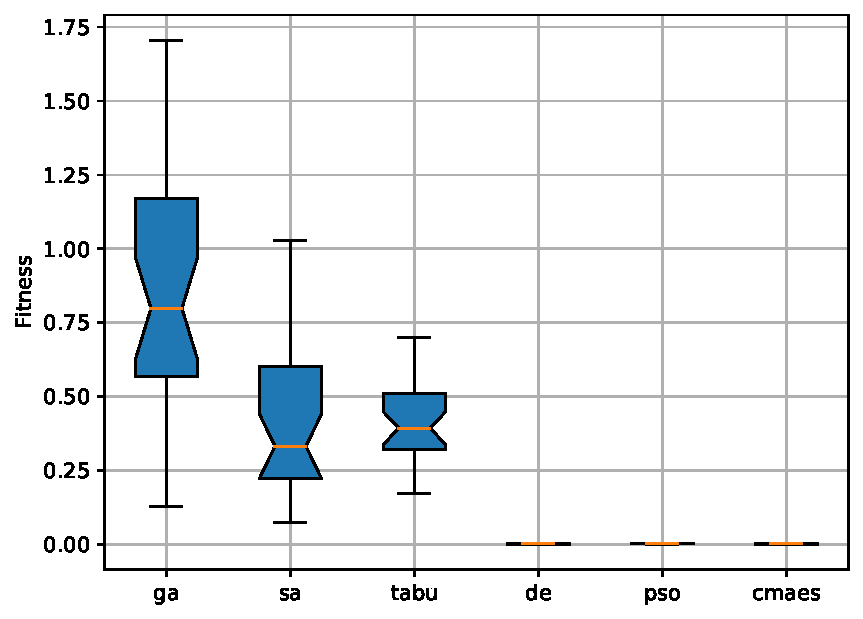
\includegraphics[width=75mm]{obrazky-figures/statistics/Validation/Ackley/JOINED/solutionsPlotsComparasion.pdf}
    &
	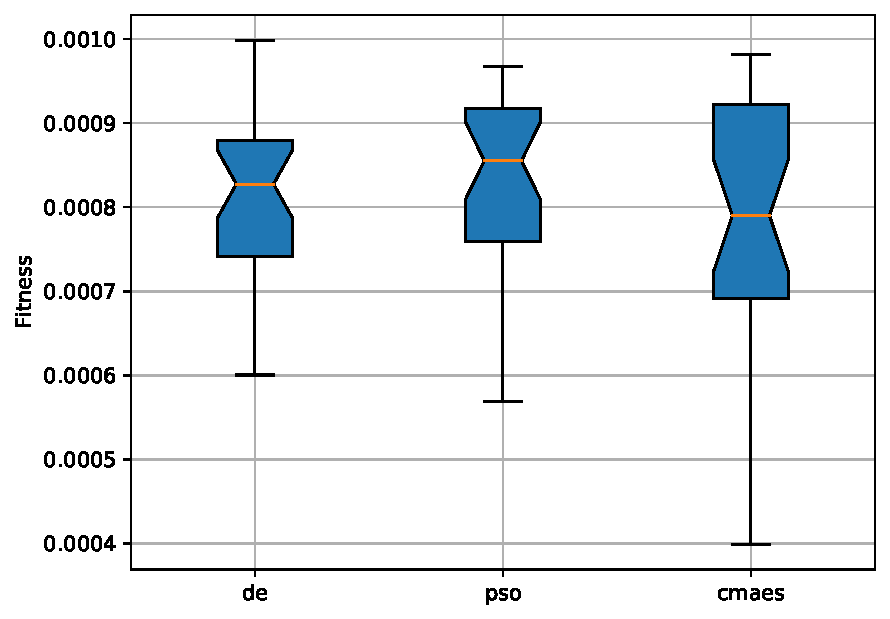
\includegraphics[width=75mm]{obrazky-figures/statistics/Validation/Ackley/JOINED/best_solutionsPlotsComparasion.pdf}
    \end{tabular}
    }
    \caption{Výsledky optimalizace Ackleyho funkce.}
    \label{fg:validation:ackley:joined}
\end{figure}

\begin{figure}[H]
    \makebox[\textwidth][c]{
    \begin{tabular}{cc}
	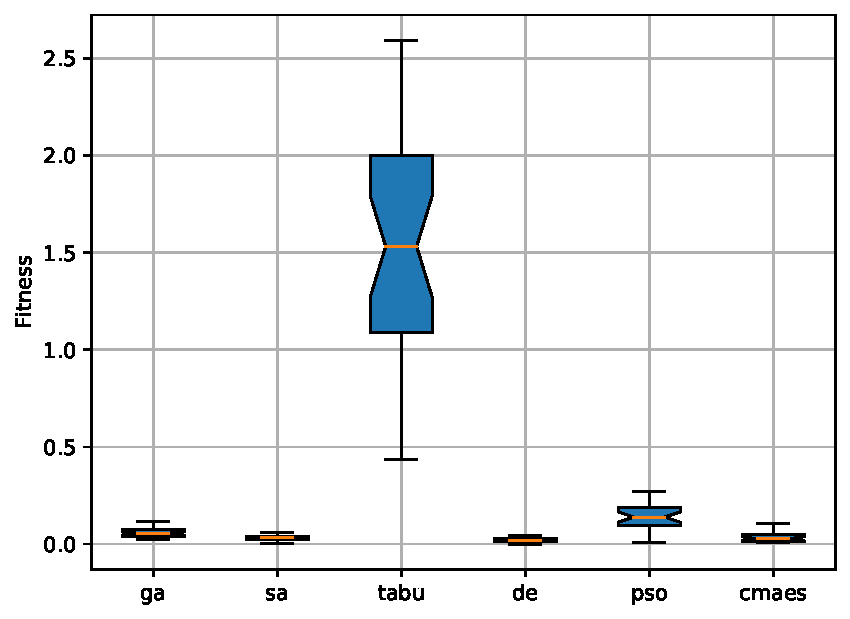
\includegraphics[width=75mm]{obrazky-figures/statistics/Validation/Griewank/JOINED/solutionsPlotsComparasion.pdf}
    &
	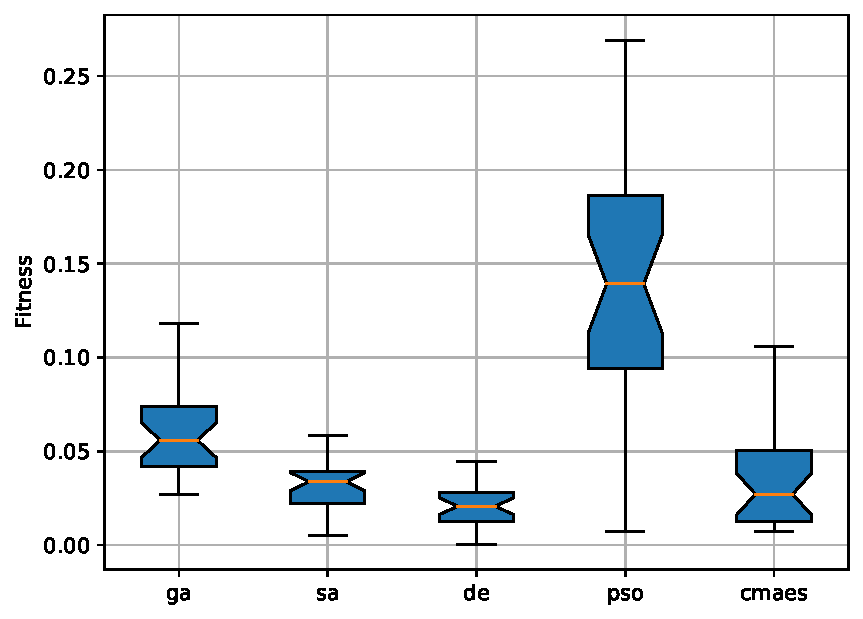
\includegraphics[width=75mm]{obrazky-figures/statistics/Validation/Griewank/JOINED/best_solutionsPlotsComparasion.pdf}
    \end{tabular}
    }
    \caption{Výsledky optimalizace Griewankovi funkce.}
    \label{fg:validation:griewank:joined}
\end{figure}

\begin{figure}[H]
    \makebox[\textwidth][c]{
    \begin{tabular}{cc}
	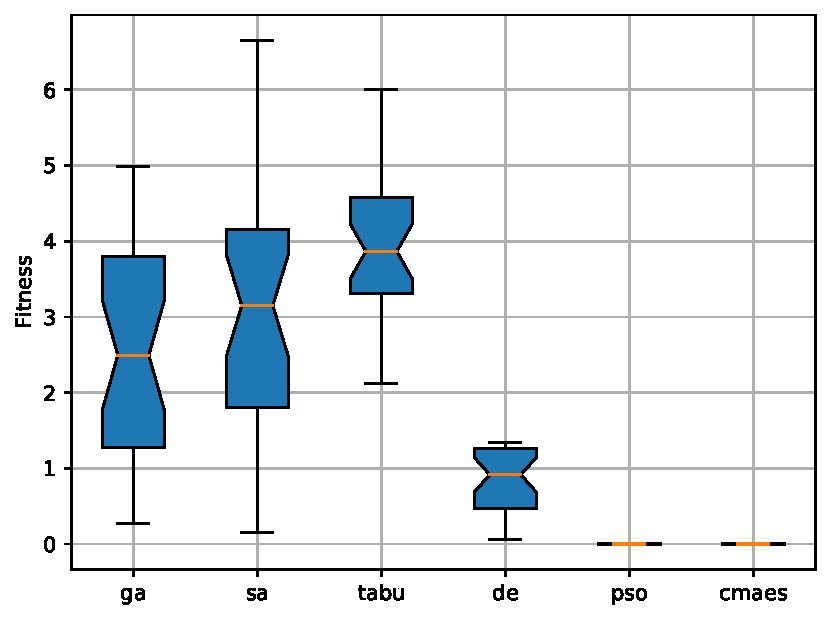
\includegraphics[width=75mm]{obrazky-figures/statistics/Validation/Rosenbrock/JOINED/solutionsPlotsComparasion.pdf}
    &
	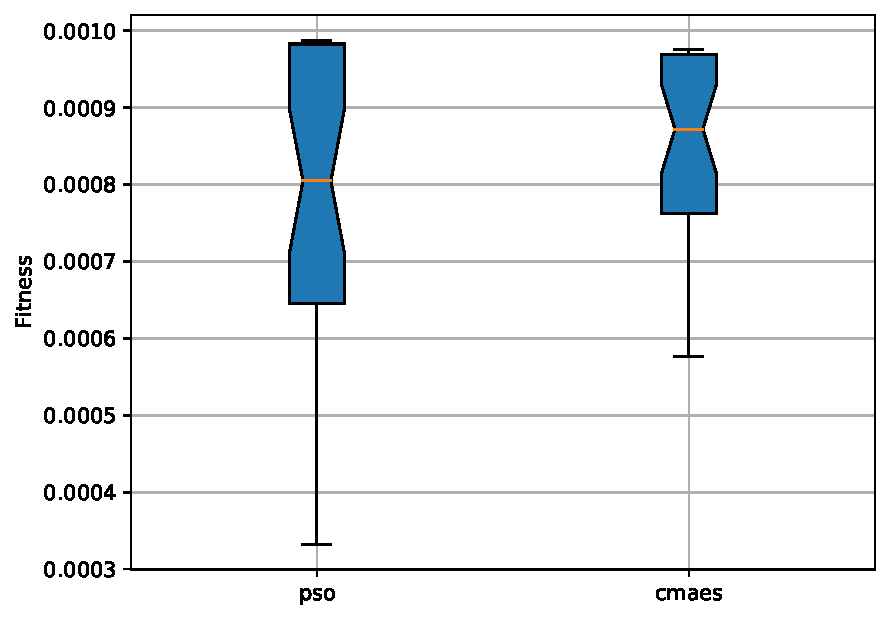
\includegraphics[width=75mm]{obrazky-figures/statistics/Validation/Rosenbrock/JOINED/best_solutionsPlotsComparasion.pdf}
    \end{tabular}
    }
    \caption{Výsledky optimalizace Rosenbrockovi funkce.}
    \label{fg:validation:rosenbrock:joined}
\end{figure}

\section{Omezené testy}
Tato sekce obsahuje statisticky zpracované data popisující průběh testů omezené optimalizace Ackleyho funkce.
\label{app:bench}
\subsection{Ackleyho funkce}
\label{app:bench:ackley}

Následující výsledky jsou agregací $30$ běhů každého optimalizačního algoritmu.
\subsubsection{Genetický algoritmus}
Pro optimalizaci byly zvoleny parametry:
\begin{itemize}
    \item Velikost populace - $64$.
    \item Turnajová selekce.
    \item Dvoubodové křížení - $80\%$.
    \item Mutace - $15\%$.
    \item Mezigenerační přežití povoleno.
\end{itemize}
Počet generací byl omezen maximálním počtem vyhodnocení fitness funkce.

\begin{figure}[H]
\begin{minipage}[t]{0.475\linewidth}
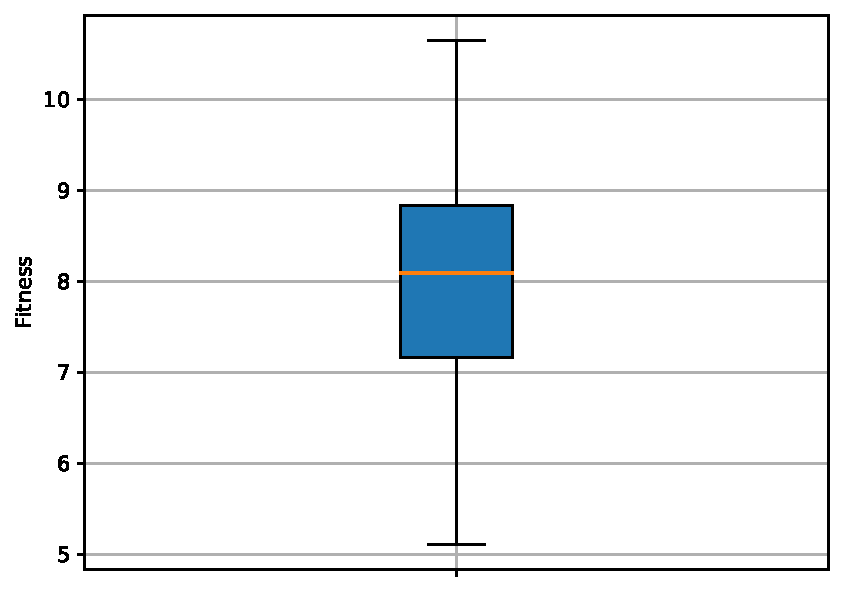
\includegraphics[width=\linewidth]{obrazky-figures/statistics/Benchmarks/Ackley/GA/bestsBoxplot_WithOutliers.pdf}
\caption{Boxplot nejlepších výsledků všech $30$ běhů GA.}
\label{fg:bench:ackley:ga:best}
\end{minipage}
\hfill
\begin{minipage}[t]{0.475\linewidth}
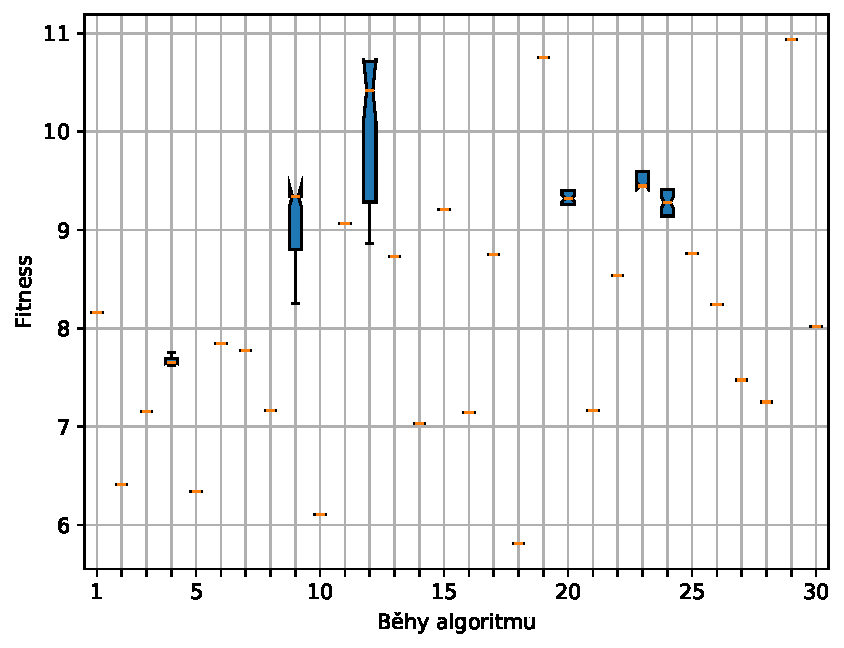
\includegraphics[width=\linewidth]{obrazky-figures/statistics/Benchmarks/Ackley/GA/lastGenBoxplots.pdf}
\caption{Boxplot stavu poslední generace všech $30$ běhů GA. Lze vidět, že populace často degenerovali.}
\label{fg:bench:ackley:ga:lastGen}
\end{minipage}
\end{figure}

\begin{figure}[H]
    \makebox[\textwidth][c]{
    \begin{tabular}{cc}
	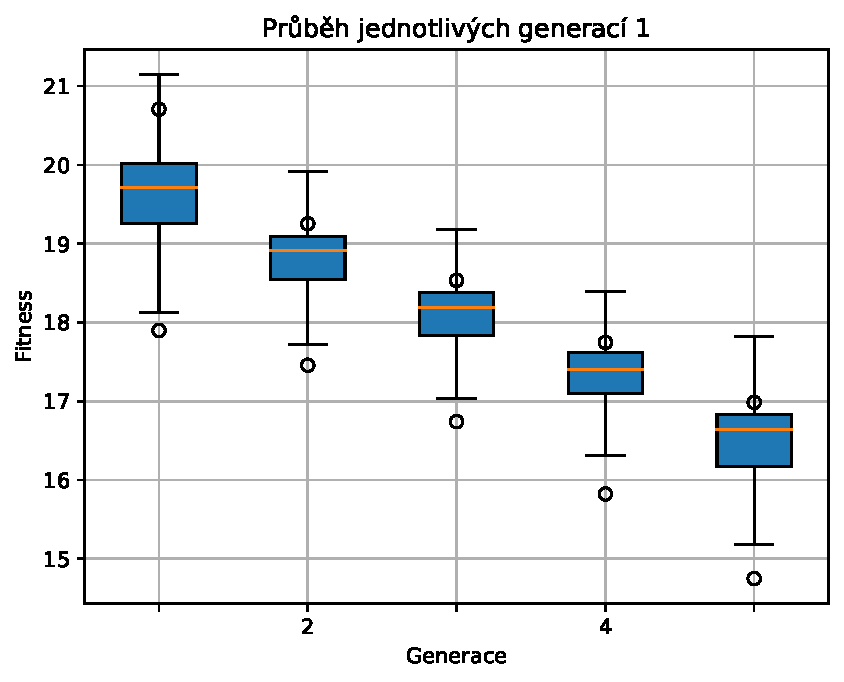
\includegraphics[width=75mm]{obrazky-figures/statistics/Benchmarks/Ackley/GA/evolutionProgress_0.pdf}
    &
	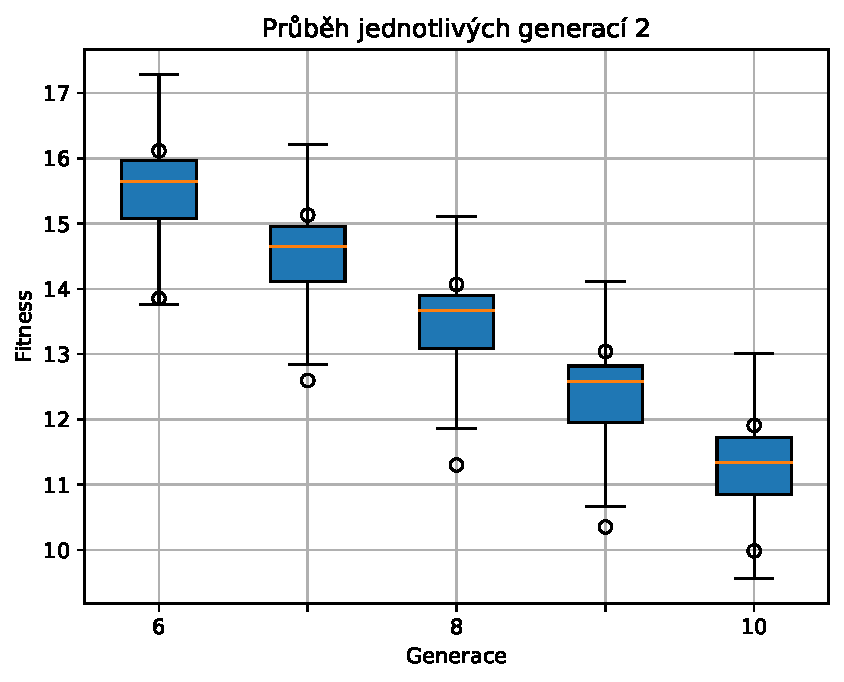
\includegraphics[width=75mm]{obrazky-figures/statistics/Benchmarks/Ackley/GA/evolutionProgress_1.pdf}
    &
	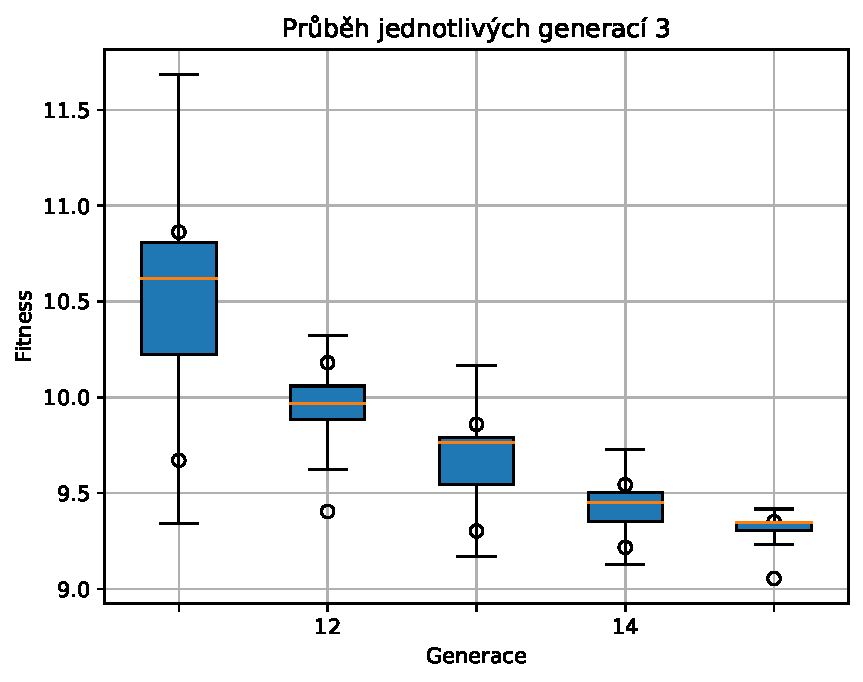
\includegraphics[width=75mm]{obrazky-figures/statistics/Benchmarks/Ackley/GA/evolutionProgress_2.pdf}
    &
	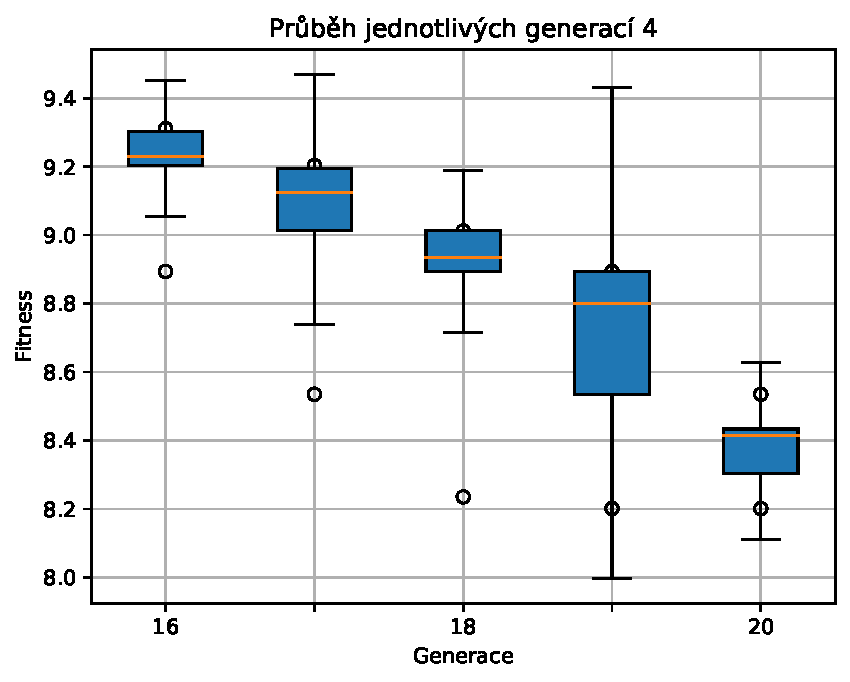
\includegraphics[width=75mm]{obrazky-figures/statistics/Benchmarks/Ackley/GA/evolutionProgress_3.pdf}
    \end{tabular}
    }
    \caption{Evoluční průběh GA. Data jsou mediány ze všech běhů v konkrétních generacích. Graf rozdělen na čtvrtiny pro větší detail. Body ukazují medián nejlepších a nejhorších nalezených řešení v dané generaci.}
    \label{fg:bench:ackley:ga:evoProg}
\end{figure}

\subsubsection{Simulované žíhání}
Pro nalezení řešení byly zvoleny následující parametry:
\begin{itemize}
    \item Počáteční teplota - $2000$.
    \item Chladící krok - $1\%$.
\end{itemize}
Teplotní rozvrh byl zvolen jako lineární. Perturberance maximálně o pětinu z rozsahu.

\begin{figure}[H]
\begin{minipage}[t]{0.475\linewidth}
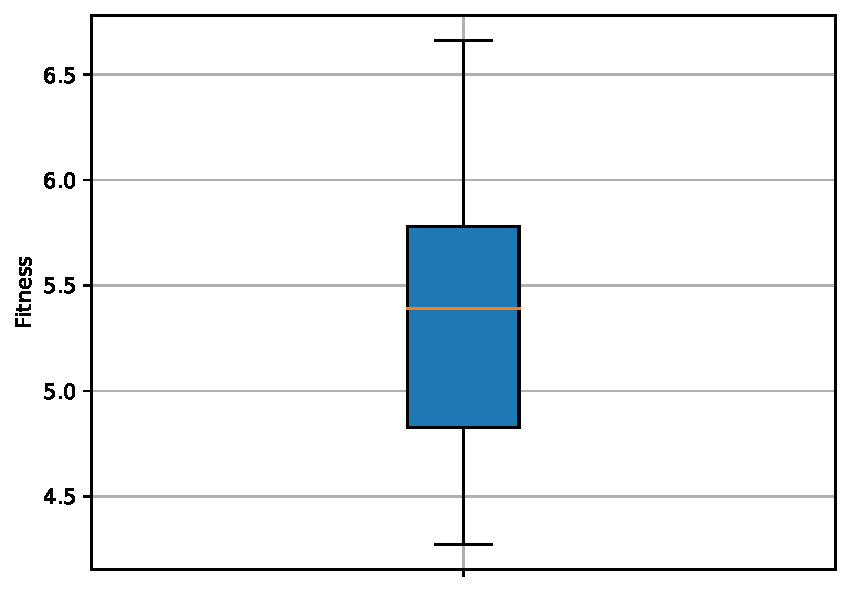
\includegraphics[width=\linewidth]{obrazky-figures/statistics/Benchmarks/Ackley/SA/bestsBoxplot_WithOutliers.pdf}
\caption{Boxplot nejlepších výsledků všech $30$ běhů SA.}
\label{fg:bench:ackley:sa:best}
\end{minipage}
\hfill
\begin{minipage}[t]{0.475\linewidth}
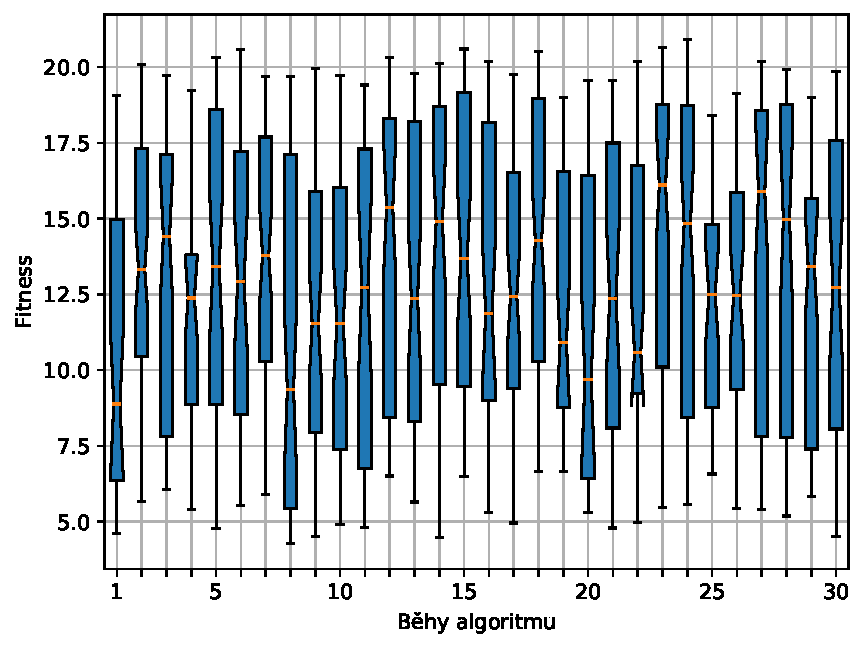
\includegraphics[width=\linewidth]{obrazky-figures/statistics/Benchmarks/Ackley/SA/lastGenBoxplots.pdf}
\caption{Boxplot fitness hodnot navštívených stavů u všech $30$ běhů SA.}
\label{fg:bench:ackley:sa:lastGen}
\end{minipage}
\end{figure}

\subsubsection{Tabu prohledávání}
Pro nalezení řešení byly zvoleny následující parametry:
\begin{itemize}
    \item Velikost tabu seznamu - $20$ stavů.
    \item Velikost prohledávaného sousedství - $5$ stavů
\end{itemize}
Použita pouze dlouhodobá paměť.

\begin{figure}[H]
\begin{minipage}[t]{0.475\linewidth}
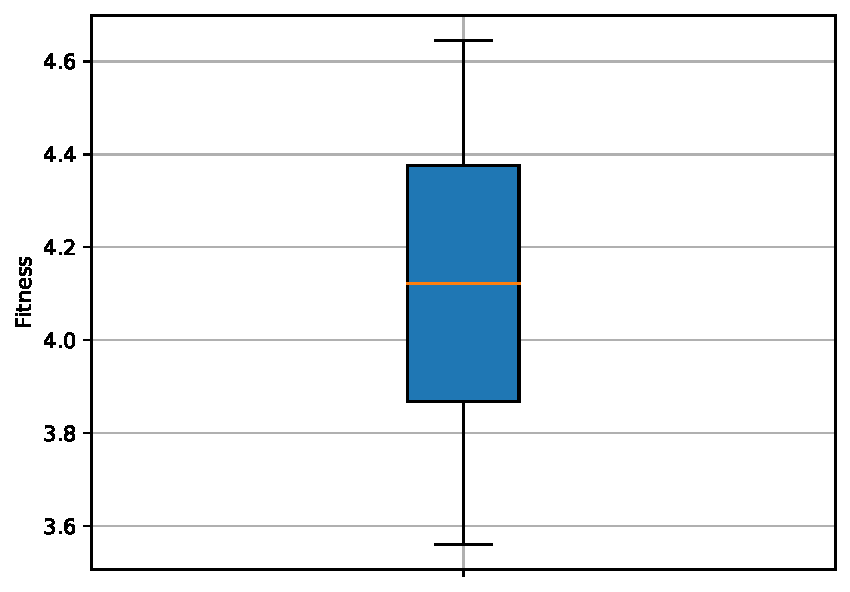
\includegraphics[width=\linewidth]{obrazky-figures/statistics/Benchmarks/Ackley/TABU/bestsBoxplot_WithOutliers.pdf}
\caption{Boxplot nejlepších výsledků všech $30$ běhů Tabu prohledávání.}
\label{fg:bench:ackley:ts:best}
\end{minipage}
\hfill
\begin{minipage}[t]{0.475\linewidth}
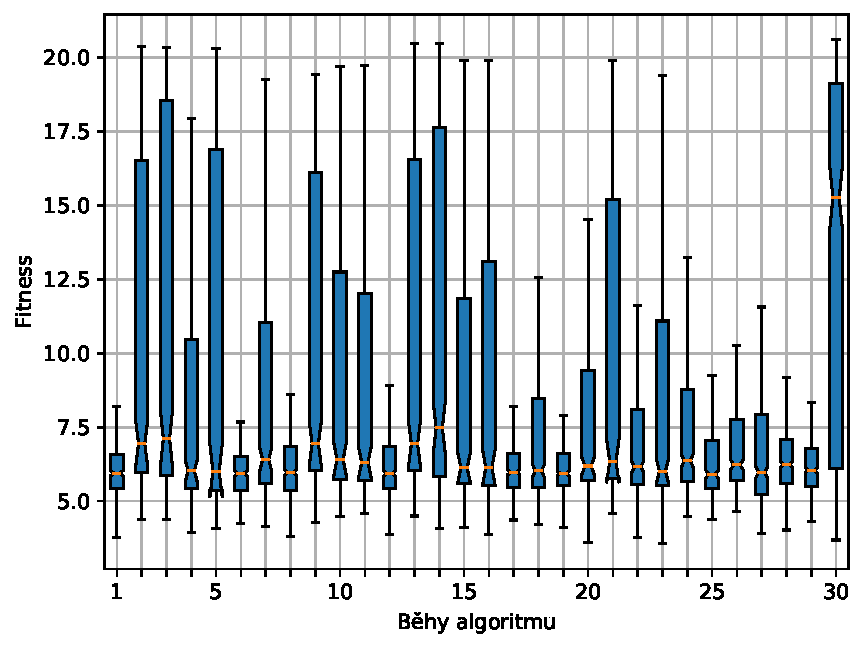
\includegraphics[width=\linewidth]{obrazky-figures/statistics/Benchmarks/Ackley/TABU/lastGenBoxplots.pdf}
\caption{Boxplot fitness hodnot navštívených stavů u všech $30$ běhů Tabu prohledávání.}
\label{fg:bench:ackley:ts:lastGen}
\end{minipage}
\end{figure}

\subsubsection{Diferenciální evoluce}
Pro nalezení řešení byly zvoleny následující parametry: 
\begin{itemize}
    \item Velikost populace - $40$.
    \item Rekombinace $80\%$.
    \item Strategie - \emph{best/1/bin}.
    \item Faktor zesílení - $0.5 - 0.9$.
\end{itemize}
Počet generací nadhodnocen tak, aby zastavení proběhlo nalezením optima nebo dosažením maximálního množství vyhodnocení fitness.

\begin{figure}[H]
\begin{minipage}[t]{0.475\linewidth}
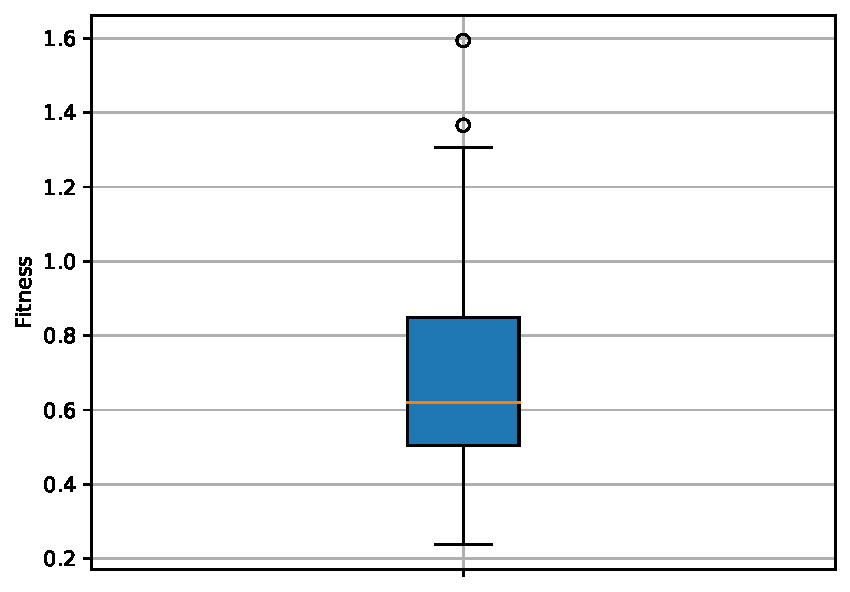
\includegraphics[width=\linewidth]{obrazky-figures/statistics/Benchmarks/Ackley/DE/bestsBoxplot_WithOutliers.pdf}
\caption{Boxplot nejlepších výsledků všech $30$ běhů DE.}
\label{fg:bench:ackley:de:best}
\end{minipage}
\hfill
\begin{minipage}[t]{0.475\linewidth}
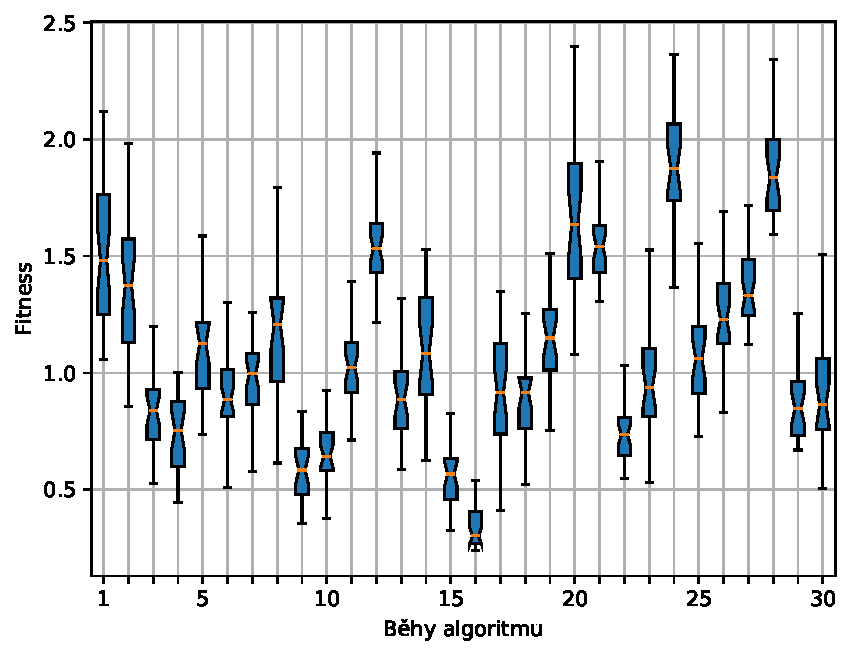
\includegraphics[width=\linewidth]{obrazky-figures/statistics/Benchmarks/Ackley/DE/lastGenBoxplots.pdf}
\caption{Boxplot stavu poslední generace všech $30$ běhů DE. Lze vidět, že populace jsou různorodé.}
\label{fg:bench:ackley:de:lastGen}
\end{minipage}
\end{figure}
\begin{figure}[H]
    \makebox[\textwidth][c]{
    \begin{tabular}{cc}
	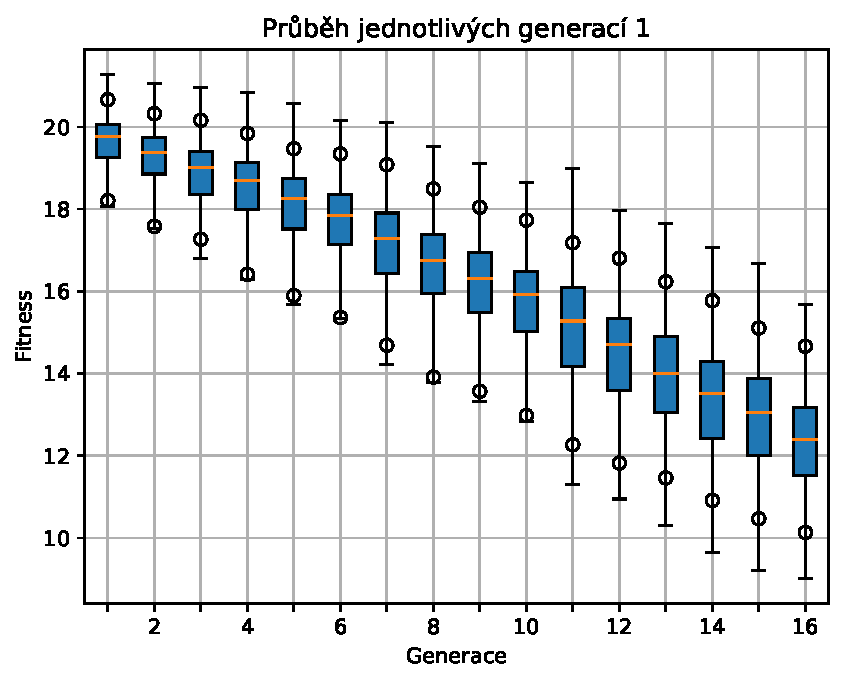
\includegraphics[width=75mm]{obrazky-figures/statistics/Benchmarks/Ackley/DE/evolutionProgress_0.pdf}
    &
	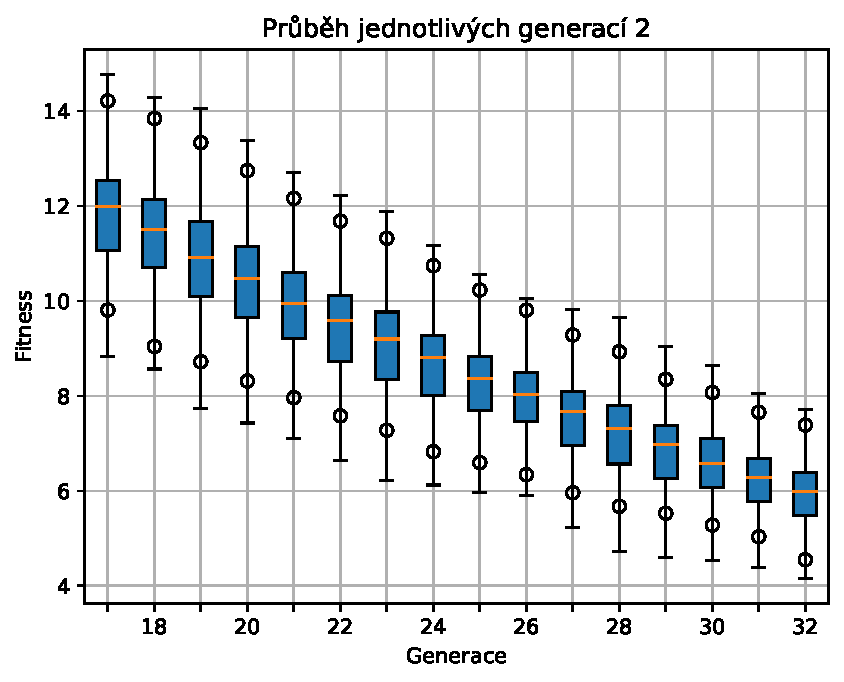
\includegraphics[width=75mm]{obrazky-figures/statistics/Benchmarks/Ackley/DE/evolutionProgress_1.pdf}
    &
	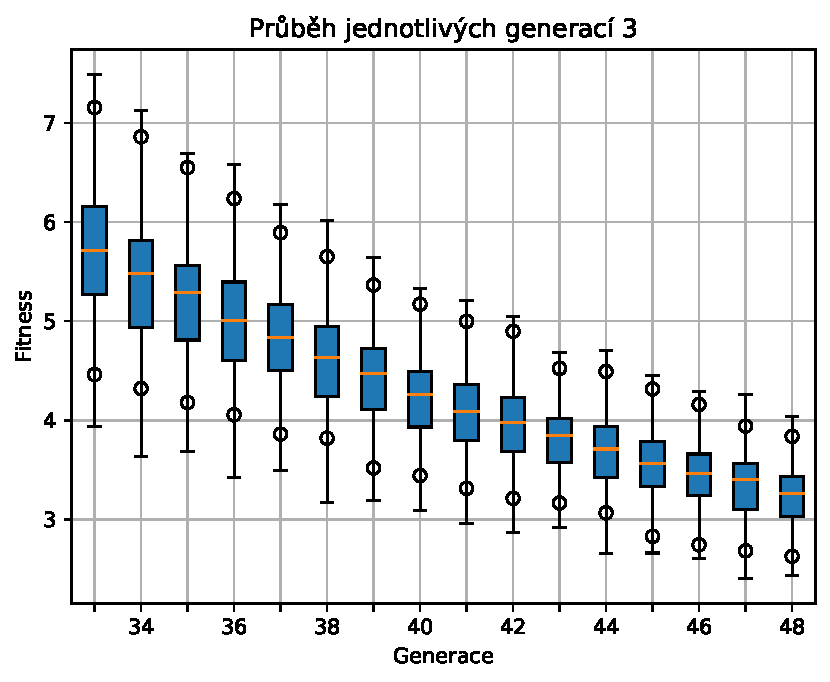
\includegraphics[width=75mm]{obrazky-figures/statistics/Benchmarks/Ackley/DE/evolutionProgress_2.pdf}
    &
	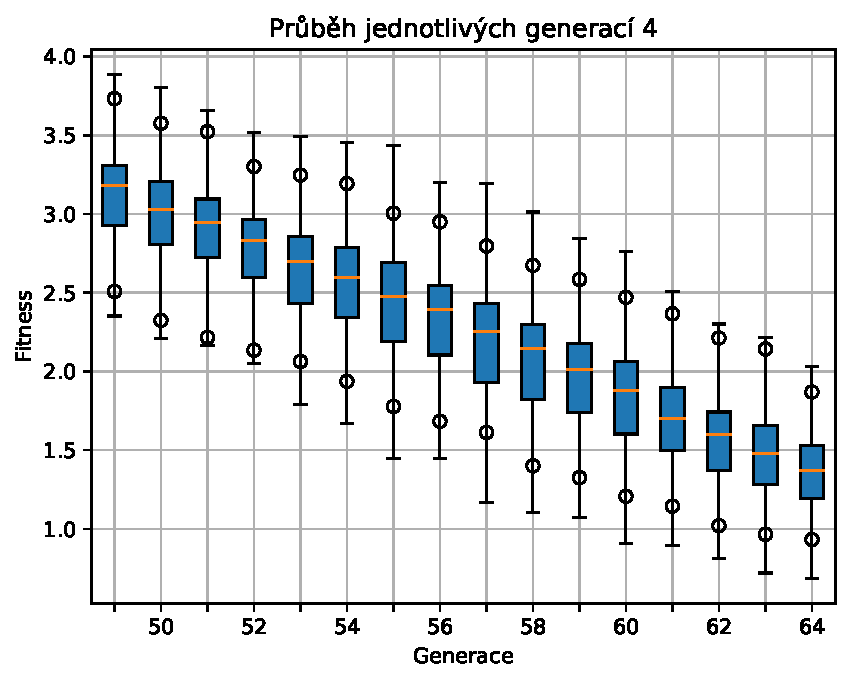
\includegraphics[width=75mm]{obrazky-figures/statistics/Benchmarks/Ackley/DE/evolutionProgress_3.pdf}
    \end{tabular}
    }
    \caption{Evoluční průběh DE. Data jsou mediány ze všech běhů v konkrétních generacích. Graf rozdělen na čtvrtiny pro větší detail. Body ukazují medián nejlepších a nejhorších nalezených řešení v dané generaci.}
    \label{fg:bench:ackley:de:evoProg}
\end{figure}
\subsubsection{Optimalizace rojem částic}
Pro optimalizaci byly použity tyto parametry:
\begin{itemize}
    \item Velikost populace - $100$ částic.
    \item Akcelerační koeficienty $c1 = c2 = 2$.
    \item Koeficient setrvačnosti $0.5$.
    \item Úplná topologie.
\end{itemize}
Počet generací nadhodnocen, aby zastavení proběhlo nalezením optima nebo dosažením maximálního množství vyhodnocení fitness.
\begin{figure}[H]
\begin{minipage}[t]{0.475\linewidth}
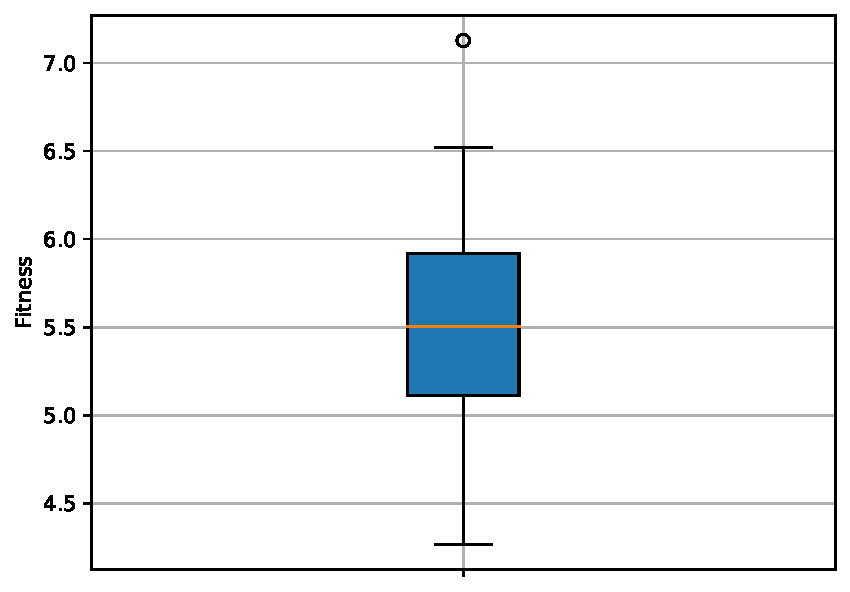
\includegraphics[width=\linewidth]{obrazky-figures/statistics/Benchmarks/Ackley/PSO/bestsBoxplot_WithOutliers.pdf}
\caption{Boxplot nejlepších výsledků všech $30$ běhů PSO.}
\label{fg:bench:ackley:pso:best}
\end{minipage}
\hfill
\begin{minipage}[t]{0.475\linewidth}
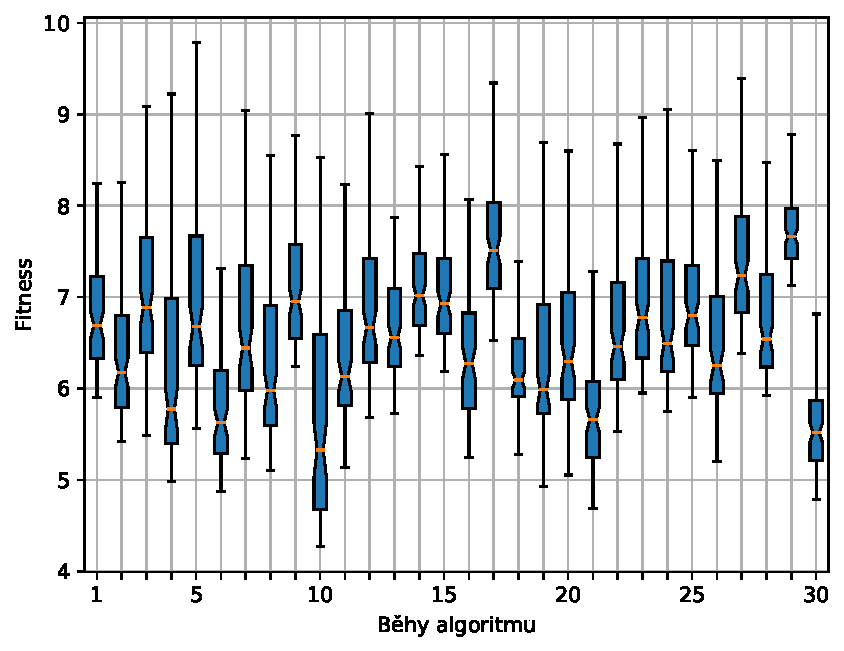
\includegraphics[width=\linewidth]{obrazky-figures/statistics/Benchmarks/Ackley/PSO/lastGenBoxplots.pdf}
\caption{Boxplot stavu poslední generace všech $30$ běhů PSO. Lze vidět, že populace jsou různorodé.}
\label{fg:bench:ackley:pso:lastGen}
\end{minipage}
\end{figure}
\begin{figure}[H]
    \makebox[\textwidth][c]{
    \begin{tabular}{cc}
	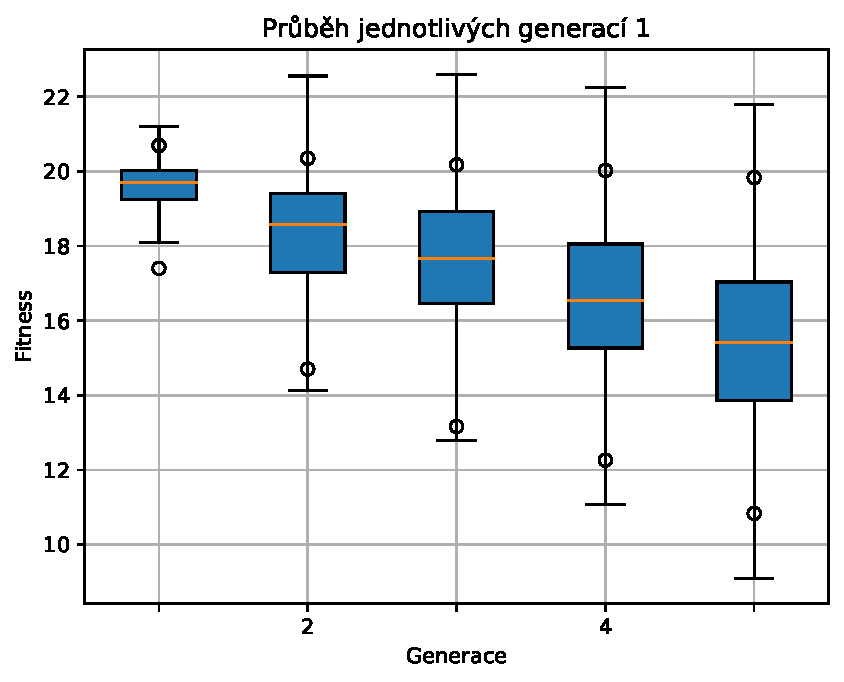
\includegraphics[width=75mm]{obrazky-figures/statistics/Benchmarks/Ackley/PSO/evolutionProgress_0.pdf}
    &
	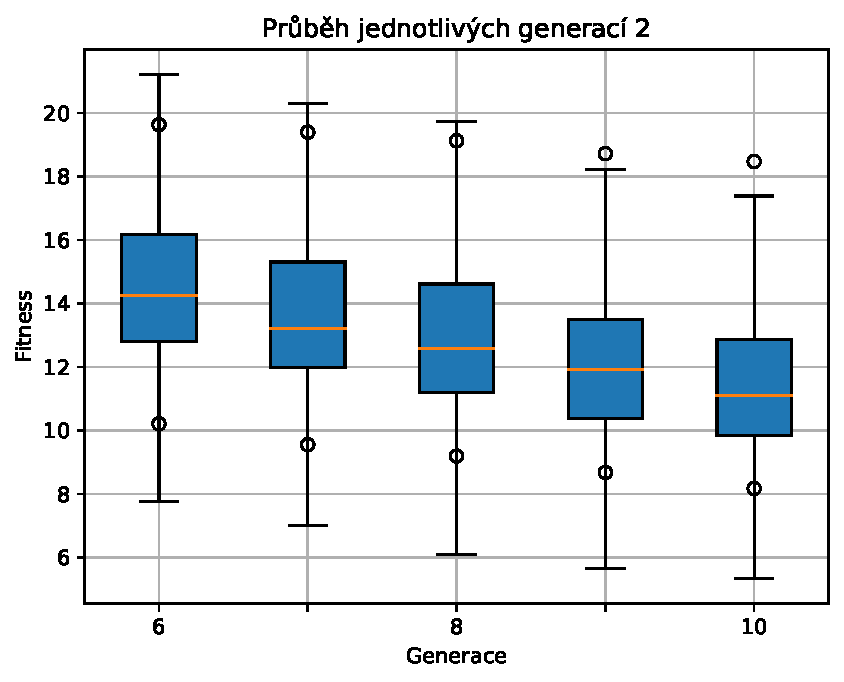
\includegraphics[width=75mm]{obrazky-figures/statistics/Benchmarks/Ackley/PSO/evolutionProgress_1.pdf}
    &
	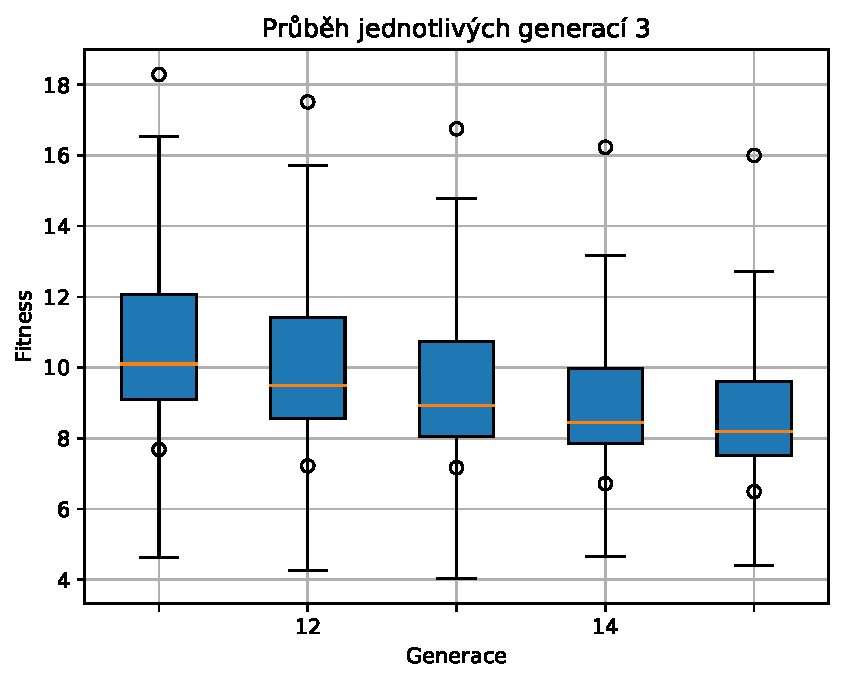
\includegraphics[width=75mm]{obrazky-figures/statistics/Benchmarks/Ackley/PSO/evolutionProgress_2.pdf}
    &
	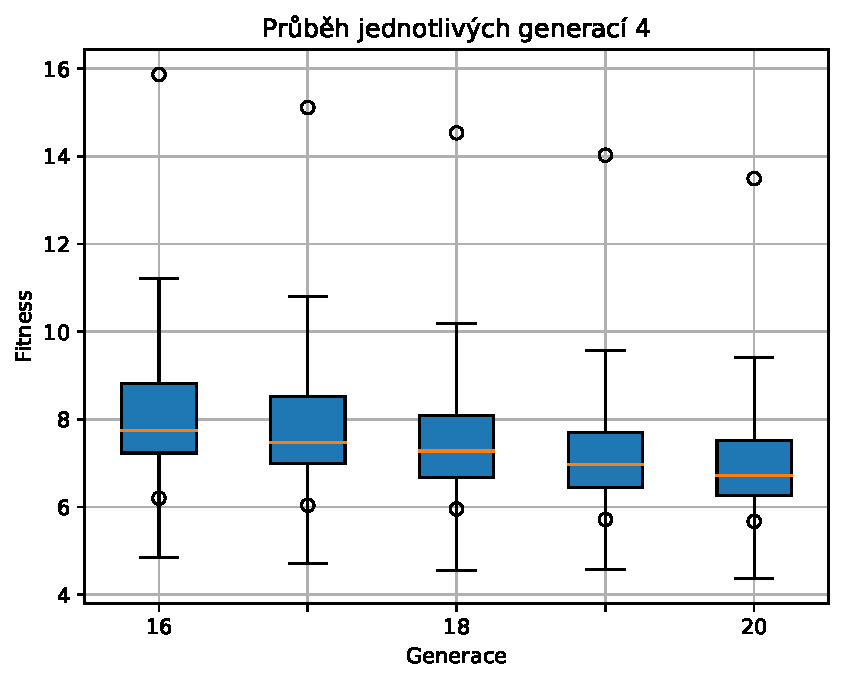
\includegraphics[width=75mm]{obrazky-figures/statistics/Benchmarks/Ackley/PSO/evolutionProgress_3.pdf}
    \end{tabular}
    }
    \caption{Evoluční průběh PSO. Data jsou mediány ze všech běhů v konkrétních generacích. Graf rozdělen na čtvrtiny pro větší detail. Body ukazují medián nejlepších a nejhorších nalezených řešení v dané generaci.}
    \label{fg:bench:ackley:pso:evoProg}
\end{figure}

\subsubsection{CMA-ES}
Výhodou \emph{CMA-ES} je skutečnost, že téměř všechny vstupní parametry jsou závislé pouze na dimenzi problému, který je předem daný. Maximální počet generací nadhodnocen, aby zastavení proběhlo nalezením optima nebo dosažením maximálního množství vyhodnocení fitness. Počáteční průměrná hodnota byla určena jako střední hodnota v mezích proměnných, standardní odchylka jako třetina absolutní hodnoty tohoto rozmezí.

\begin{figure}[H]
\begin{minipage}[t]{0.475\linewidth}
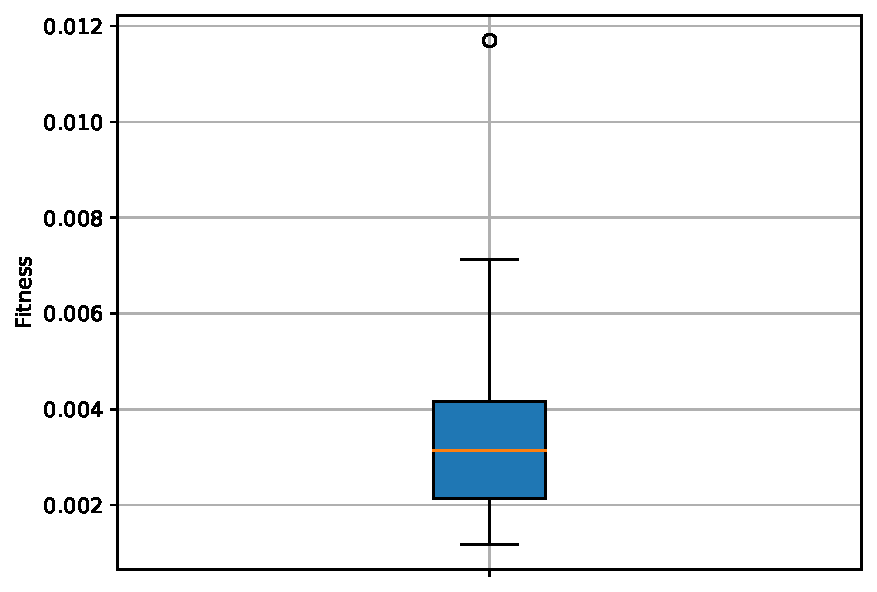
\includegraphics[width=\linewidth]{obrazky-figures/statistics/Benchmarks/Ackley/CMAES/bestsBoxplot_WithOutliers.pdf}
\caption{Boxplot nejlepších výsledků všech $30$ běhů CMA-ES.}
\label{fg:bench:ackley:cmaes:best}
\end{minipage}
\hfill
\begin{minipage}[t]{0.475\linewidth}
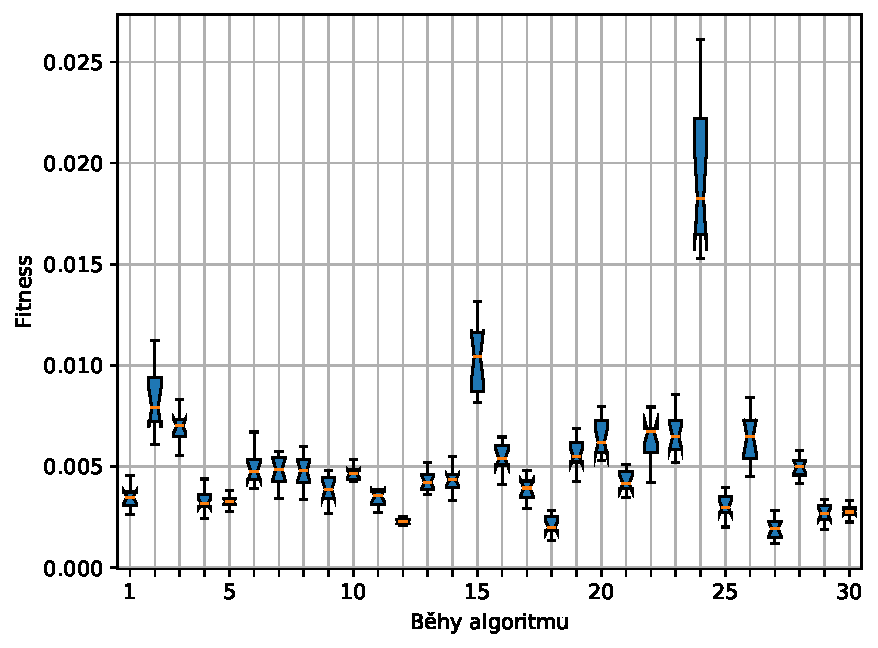
\includegraphics[width=\linewidth]{obrazky-figures/statistics/Benchmarks/Ackley/CMAES/lastGenBoxplots.pdf}
\caption{Boxplot stavu poslední generace všech $30$ běhů CMA-ES. Lze vidět, že populace jsou různorodé.}
\label{fg:bench:ackley:cmaes:lastGen}
\end{minipage}
\end{figure}
\begin{figure}[H]
    \makebox[\textwidth][c]{
    \begin{tabular}{cc}
	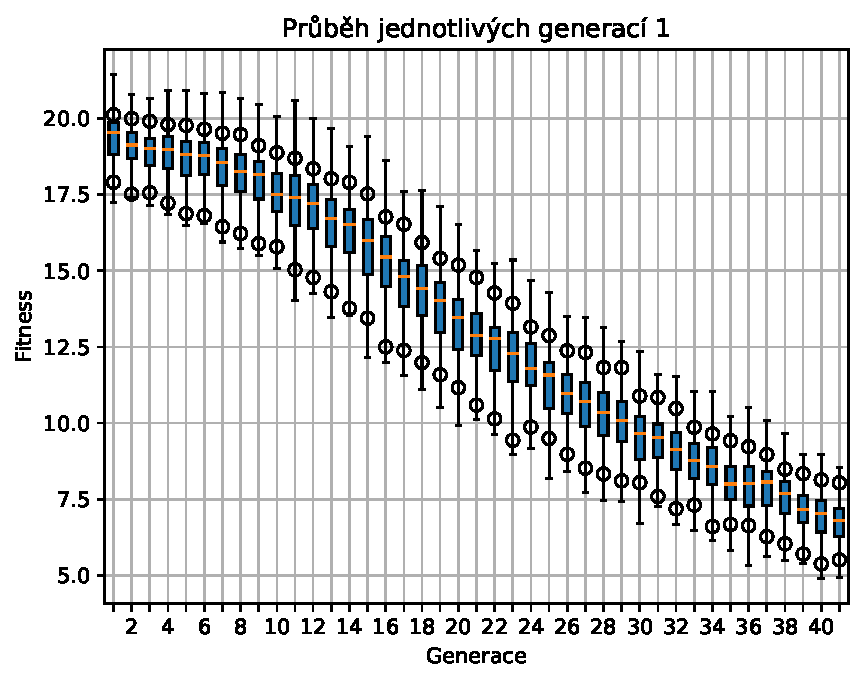
\includegraphics[width=75mm]{obrazky-figures/statistics/Benchmarks/Ackley/CMAES/evolutionProgress_0.pdf}
    &
	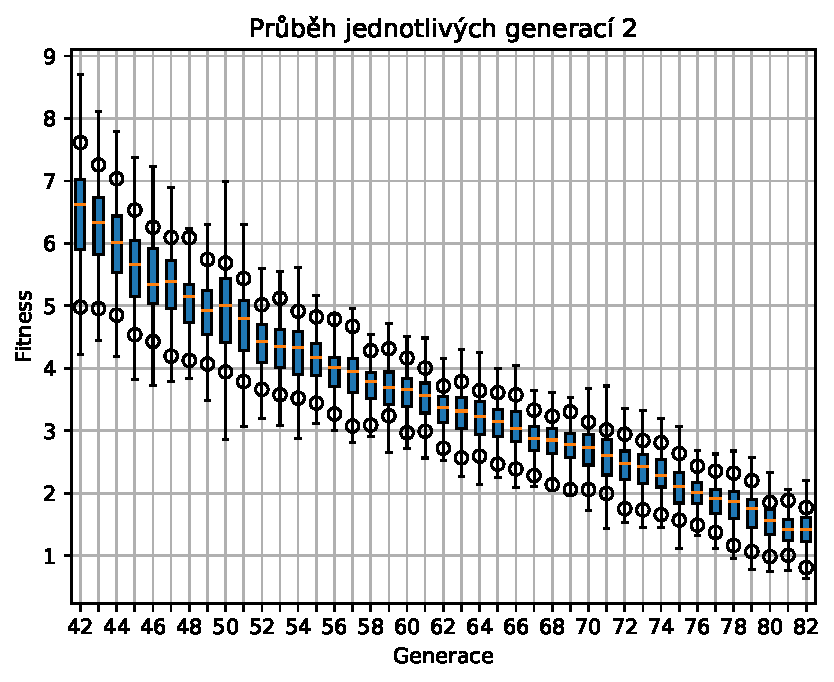
\includegraphics[width=75mm]{obrazky-figures/statistics/Benchmarks/Ackley/CMAES/evolutionProgress_1.pdf}
    &
	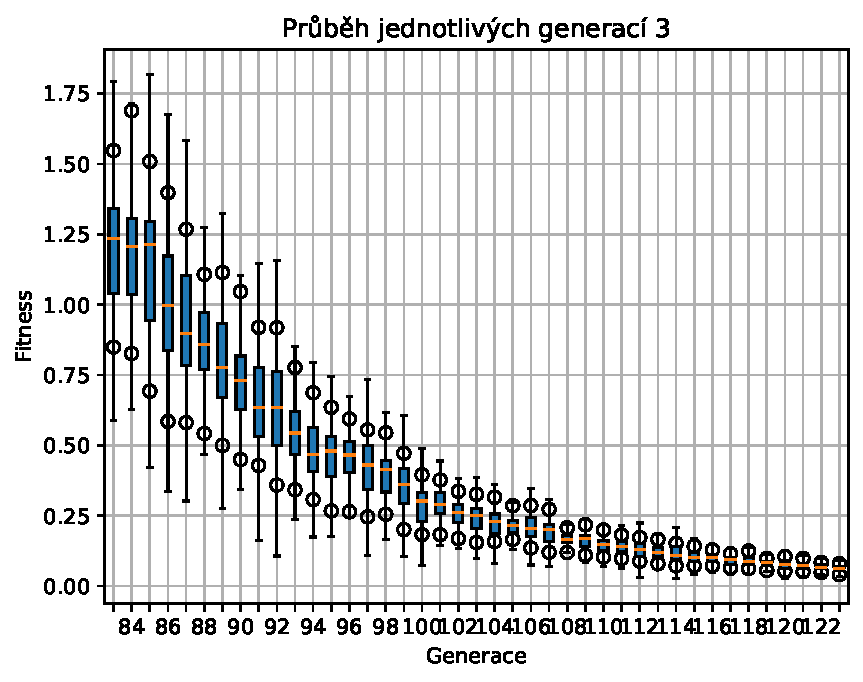
\includegraphics[width=75mm]{obrazky-figures/statistics/Benchmarks/Ackley/CMAES/evolutionProgress_2.pdf}
    &
	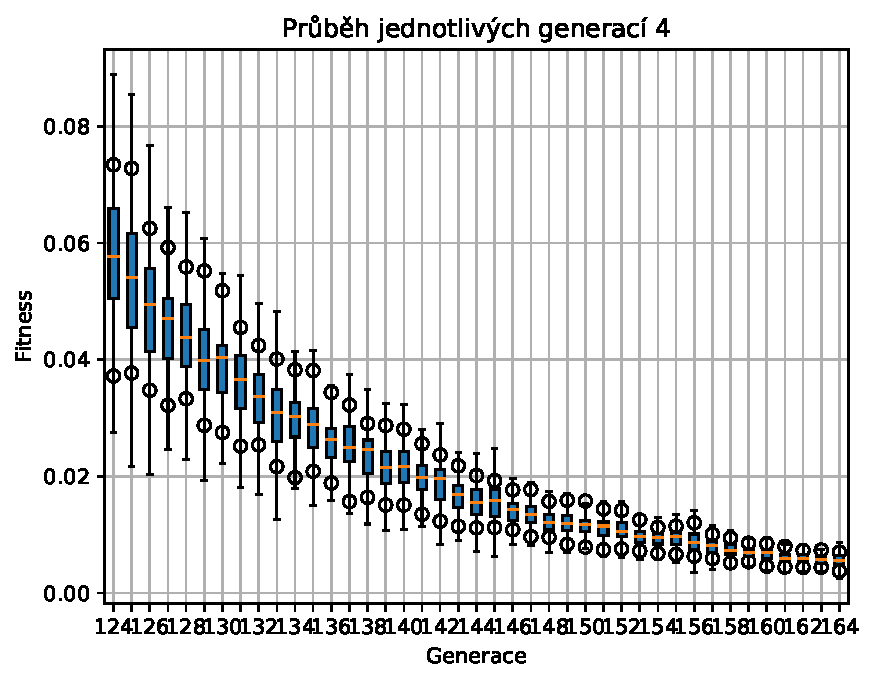
\includegraphics[width=75mm]{obrazky-figures/statistics/Benchmarks/Ackley/CMAES/evolutionProgress_3.pdf}
    \end{tabular}
    }
    \caption{Evoluční průběh CMA-ES. Data jsou mediány ze všech běhů v konkrétních generacích. Graf rozdělen na čtvrtiny pro větší detail. Body ukazují medián nejlepších a nejhorších nalezených řešení v dané generaci.}
    \label{fg:bench:ackley:cmaes:evoProg}
\end{figure}






\subsection{Griewankova funkce}
\label{app:bench:griew}

Statisticky zpracované výsledky $30$ běhů každého optimalizačního algoritmu.
\subsubsection{Genetický algoritmus}
Pro optimalizace byly použity následující parametry:
\begin{itemize}
    \item Velikost populace - $50$.
    \item Turnajový výběr.
    \item Dvoubodové křížení - $80\%$.
    \item Mutace - $20\%$.
    \item Přežití nejlepších bez ohledu na generaci.
\end{itemize}
Maximální počet generací nadhodnocen, aby zastavení proběhlo nalezením optima nebo dosažením maximálního množství vyhodnocení fitness.

\begin{figure}[H]
\begin{minipage}[t]{0.475\linewidth}
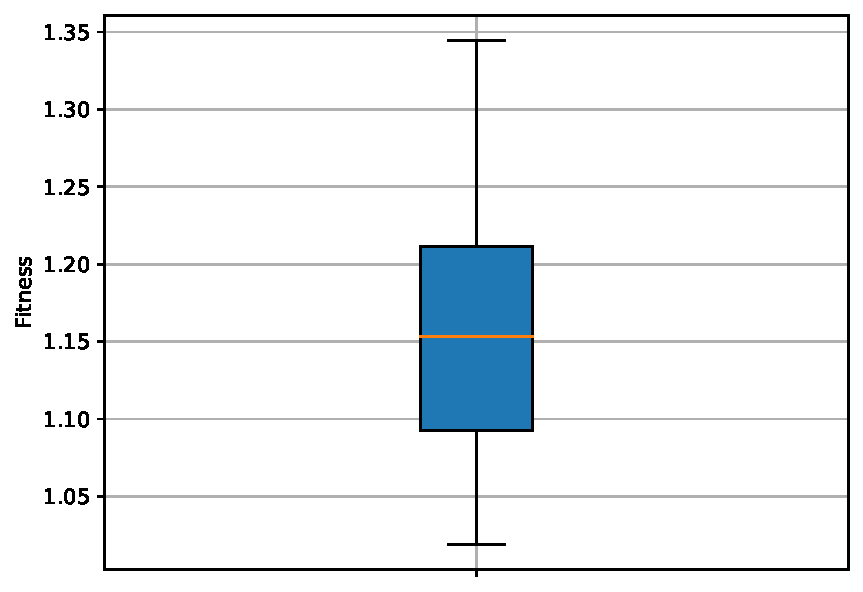
\includegraphics[width=\linewidth]{obrazky-figures/statistics/Benchmarks/Griewank/GA/bestsBoxplot_WithOutliers.pdf}
\caption{Boxplot nejlepších výsledků všech $30$ běhů GA.}
\label{fg:bench:griewank:ga:best}
\end{minipage}
\hfill
\begin{minipage}[t]{0.475\linewidth}
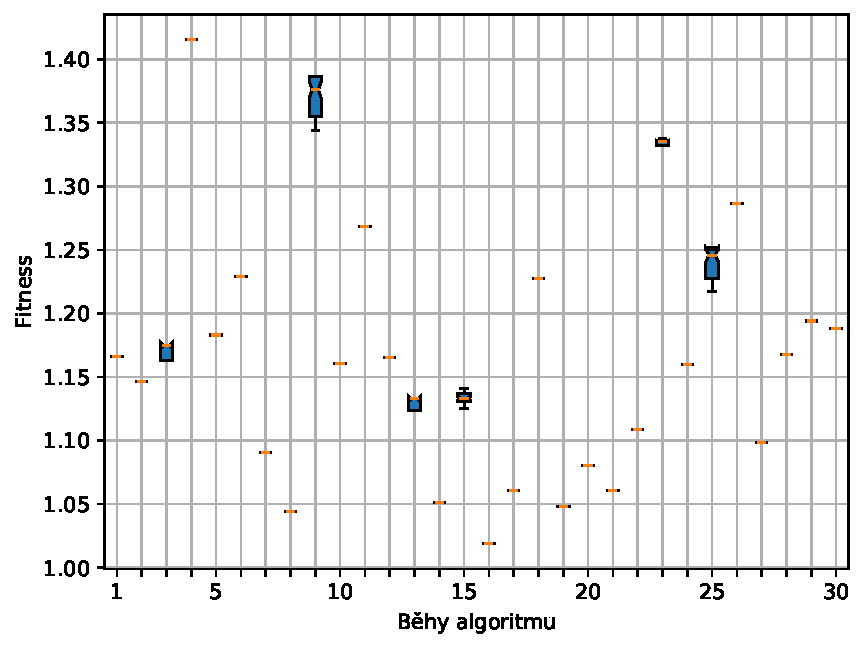
\includegraphics[width=\linewidth]{obrazky-figures/statistics/Benchmarks/Griewank/GA/lastGenBoxplots.pdf}
\caption{Boxplot stavu poslední generace všech $30$ běhů GA.}
\label{fg:bench:griewank:ga:lastGen}
\end{minipage}
\end{figure}

\begin{figure}[H]
    \makebox[\textwidth][c]{
    \begin{tabular}{cc}
	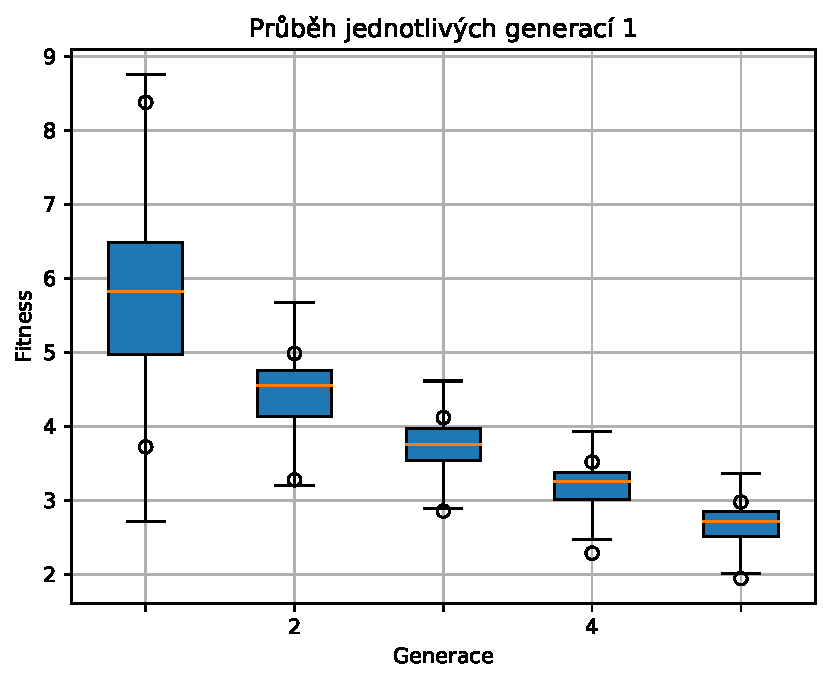
\includegraphics[width=75mm]{obrazky-figures/statistics/Benchmarks/Griewank/GA/evolutionProgress_0.pdf}
    &
	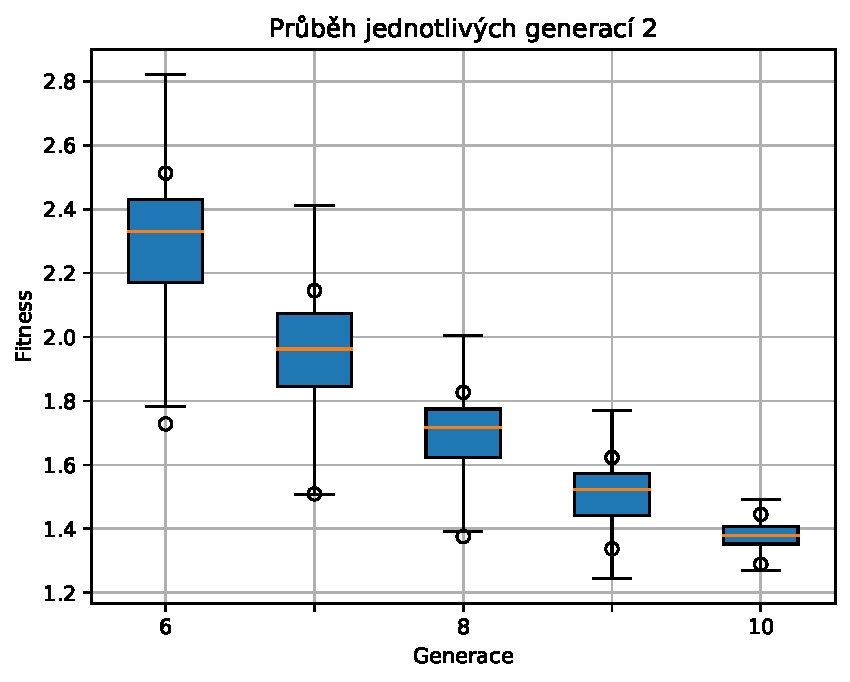
\includegraphics[width=75mm]{obrazky-figures/statistics/Benchmarks/Griewank/GA/evolutionProgress_1.pdf}
    &
	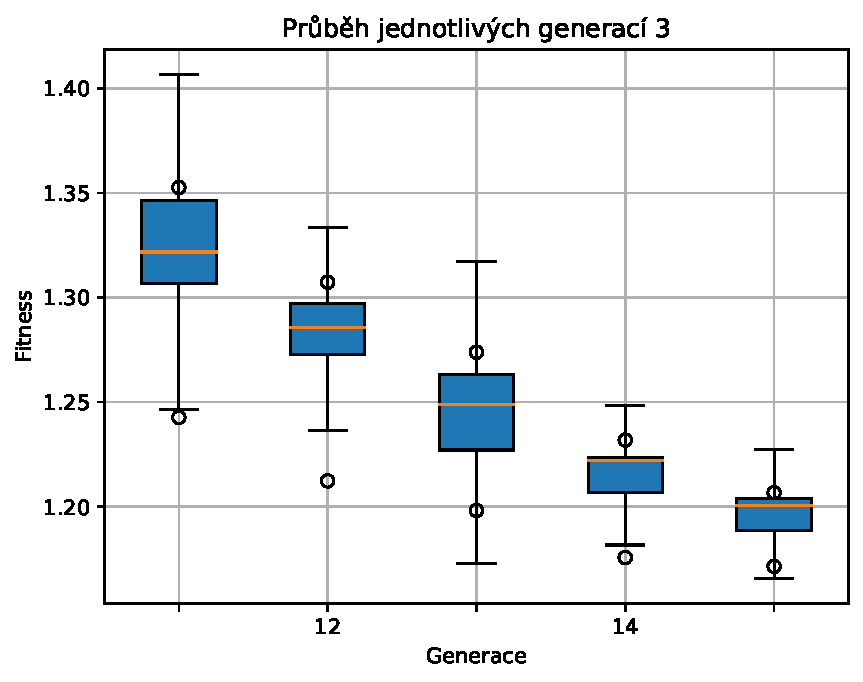
\includegraphics[width=75mm]{obrazky-figures/statistics/Benchmarks/Griewank/GA/evolutionProgress_2.pdf}
    &
	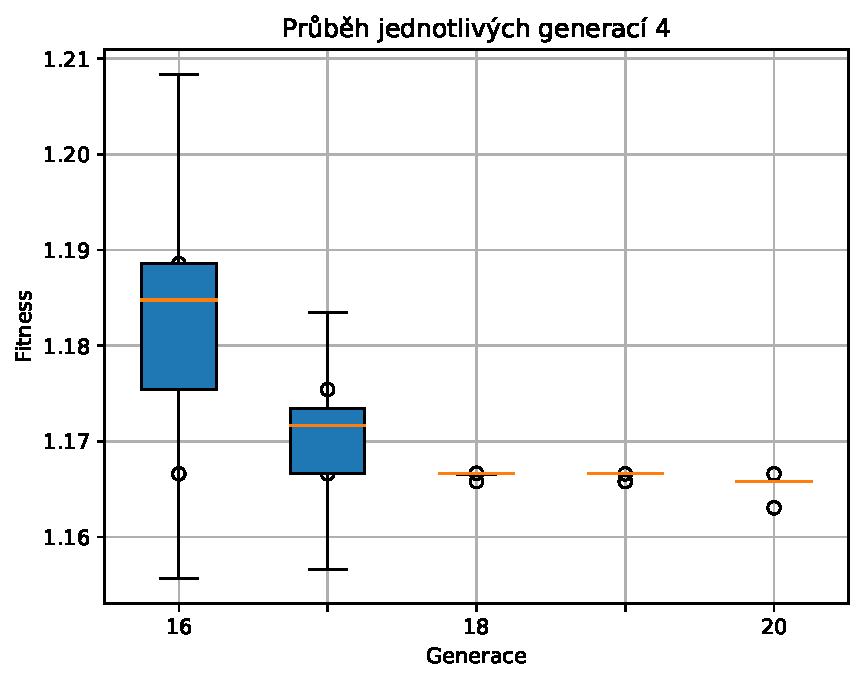
\includegraphics[width=75mm]{obrazky-figures/statistics/Benchmarks/Griewank/GA/evolutionProgress_3.pdf}
    \end{tabular}
    }
    \caption{Evoluční průběh GA. Data jsou mediány ze všech běhů v konkrétních generacích. Graf rozdělen na čtvrtiny pro větší detail. Body ukazují medián nejlepších a nejhorších nalezených řešení v dané generaci.}
    \label{fg:bench:griewank:ga:evoProg}
\end{figure}

\subsubsection{Simulované žíhání}
Pro nejoptimálnější řešení byly nalezeny parametry 
\begin{itemize}
    \item Počáteční teplota - $2000$
    \item Chladící krok - $1\%$
\end{itemize}
Teplotní rozvrh byl zvolen jako lineární. Perturberance stavu je o číslo z Gaussova rozložení s průměrem 0 a odchylkou pětina rozmezí prostoru proměnné.

\begin{figure}[H]
\begin{minipage}[t]{0.475\linewidth}
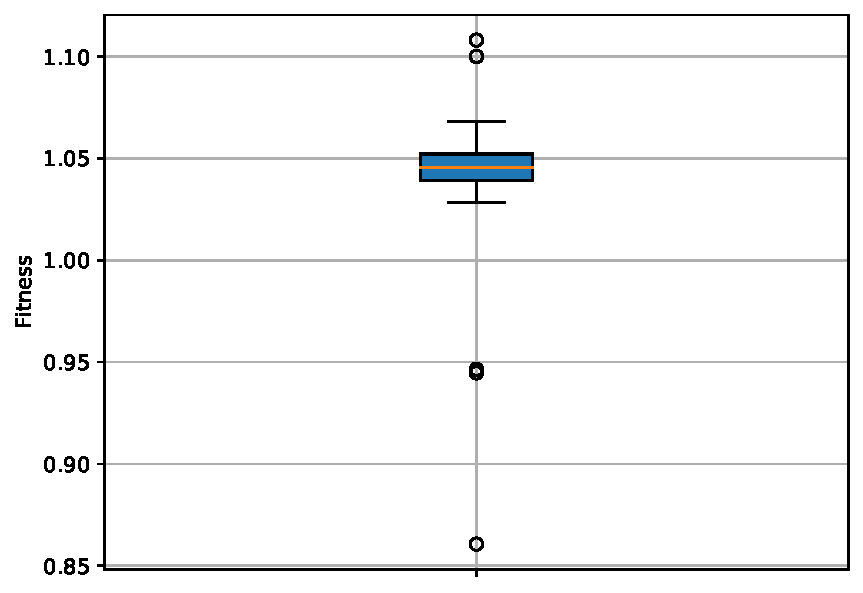
\includegraphics[width=\linewidth]{obrazky-figures/statistics/Benchmarks/Griewank/SA/bestsBoxplot_WithOutliers.pdf}
\caption{Boxplot nejlepších výsledků všech $30$ běhů SA.}
\label{fg:bench:griewank:sa:best}
\end{minipage}
\hfill
\begin{minipage}[t]{0.475\linewidth}
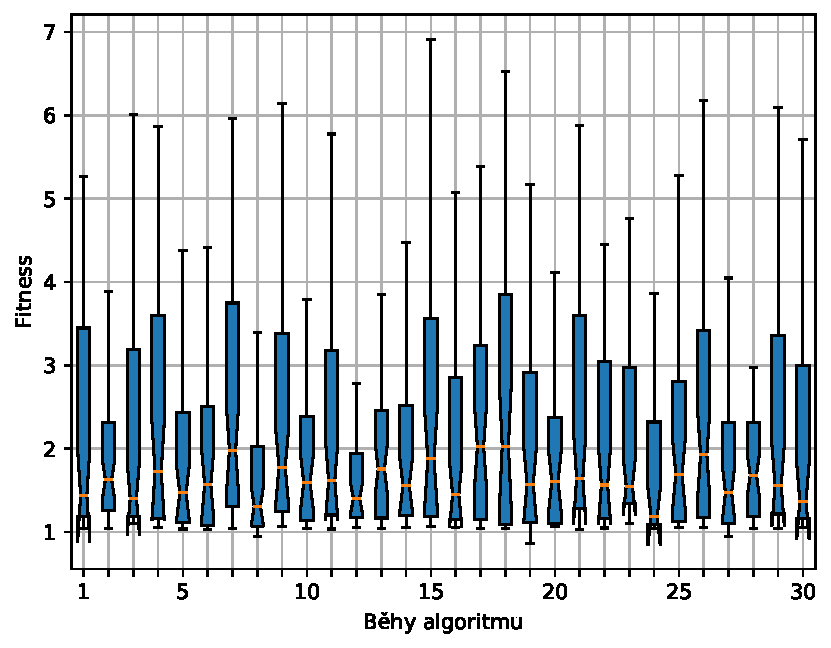
\includegraphics[width=\linewidth]{obrazky-figures/statistics/Benchmarks/Griewank/SA/lastGenBoxplots.pdf}
\caption{Boxplot stavu poslední generace všech $30$ běhů SA.}
\label{fg:bench:griewank:sa:lastGen}
\end{minipage}
\end{figure}

\subsubsection{Tabu prohledávání}
Pro nalezení řešení byly zvoleny následující parametry:
\begin{itemize}
    \item Velikost tabu seznamu - $20$
    \item Velikost prohledávaného sousedství - $5$
\end{itemize}
Použita pouze dlouhodobá paměť.

\begin{figure}[H]
\begin{minipage}[t]{0.475\linewidth}
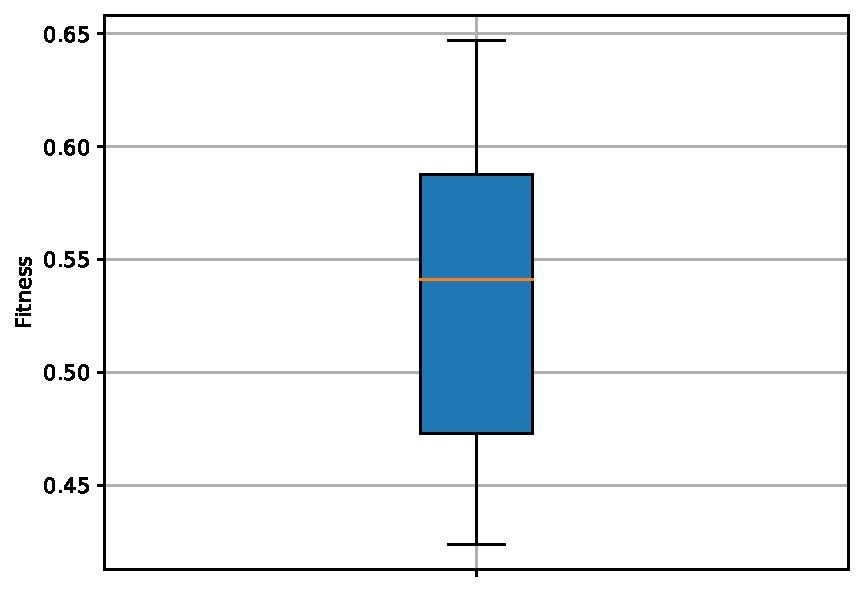
\includegraphics[width=\linewidth]{obrazky-figures/statistics/Benchmarks/Griewank/TABU/bestsBoxplot_WithOutliers.pdf}
\caption{Boxplot nejlepších výsledků všech $30$ běhů Tabu prohledávání.}
\label{fg:bench:griewank:tabu:best}
\end{minipage}
\hfill
\begin{minipage}[t]{0.475\linewidth}
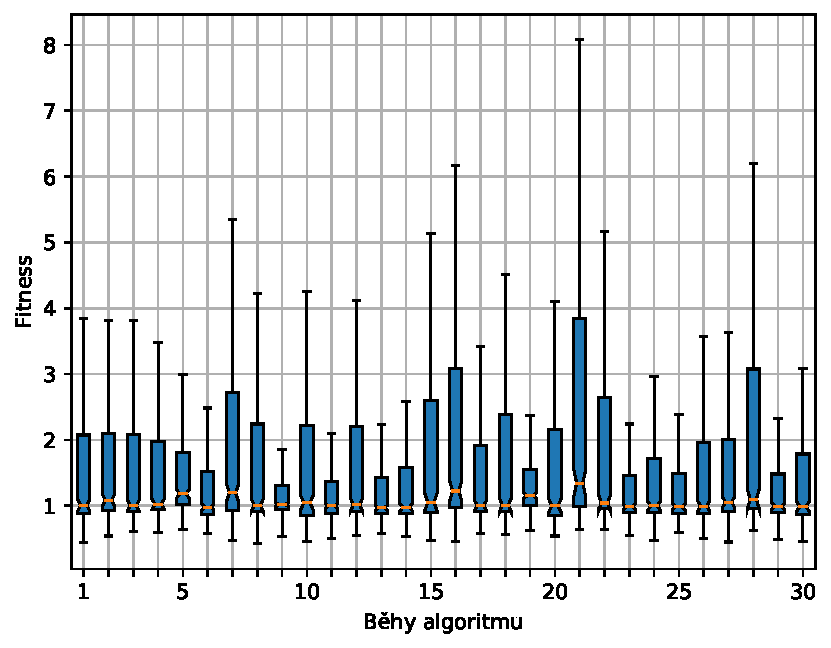
\includegraphics[width=\linewidth]{obrazky-figures/statistics/Benchmarks/Griewank/TABU/lastGenBoxplots.pdf}
\caption{Boxplot stavu poslední generace všech $30$ běhů Tabu prohledávání.}
\label{fg:bench:griewank:tabu:lastGen}
\end{minipage}
\end{figure}

\subsubsection{Diferenciální evoluce}
Pro optimalizaci byly použity tyto parametry:
\begin{itemize}
    \item Velikost populace - $40$.
    \item Rekombinace - $75\%$.
    \item Strategie \emph{rand-to-best/1/bin}.
    \item Faktor zesílení $0.5$.
\end{itemize}
I zde byl počet generací nadhodnocen tak, aby zastavení proběhlo nalezením optima nebo dosažením maximálního množství vyhodnocení fitness.

\begin{figure}[H]
\begin{minipage}[t]{0.475\linewidth}
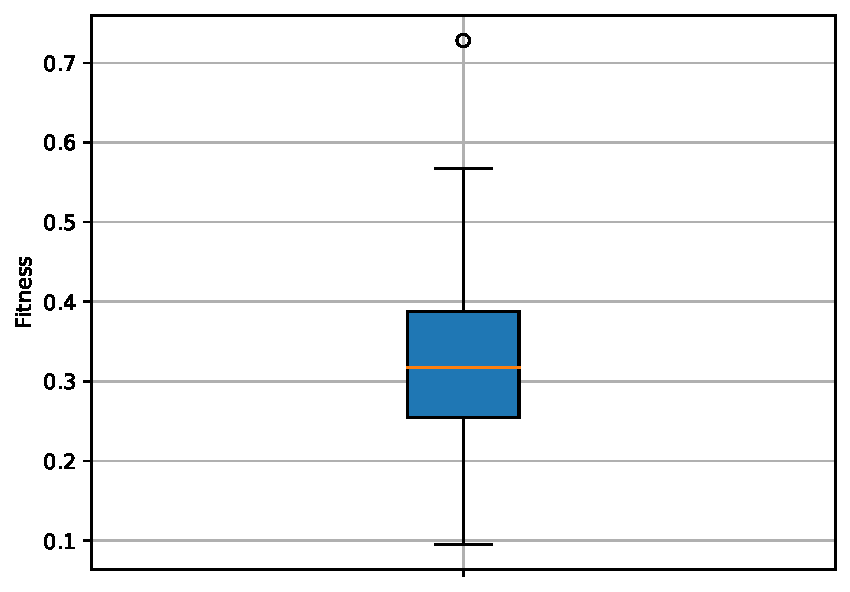
\includegraphics[width=\linewidth]{obrazky-figures/statistics/Benchmarks/Griewank/DE/bestsBoxplot_WithOutliers.pdf}
\caption{Boxplot nejlepších výsledků všech $30$ běhů DE.}
\label{fg:bench:griewank:de:best}
\end{minipage}
\hfill
\begin{minipage}[t]{0.475\linewidth}
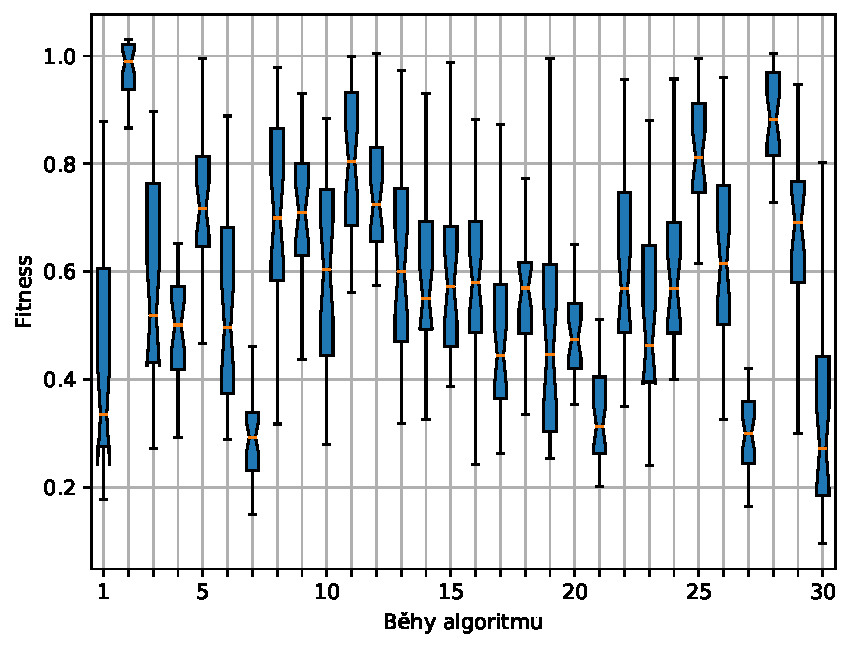
\includegraphics[width=\linewidth]{obrazky-figures/statistics/Benchmarks/Griewank/DE/lastGenBoxplots.pdf}
\caption{Boxplot stavu poslední generace všech $30$ běhů DE.}
\label{fg:bench:griewank:gdea:lastGen}
\end{minipage}
\end{figure}

\begin{figure}[H]
    \makebox[\textwidth][c]{
    \begin{tabular}{cc}
	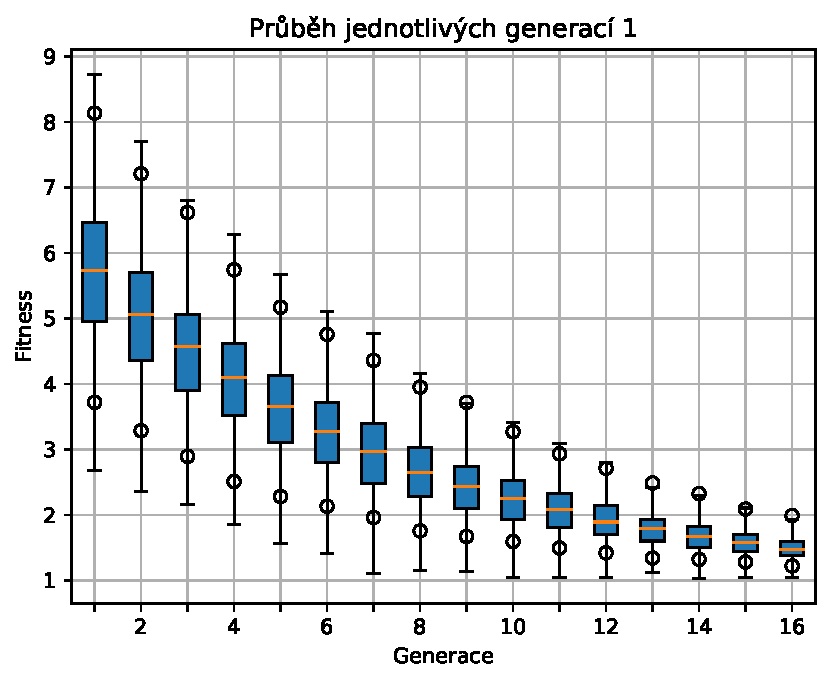
\includegraphics[width=75mm]{obrazky-figures/statistics/Benchmarks/Griewank/DE/evolutionProgress_0.pdf}
    &
	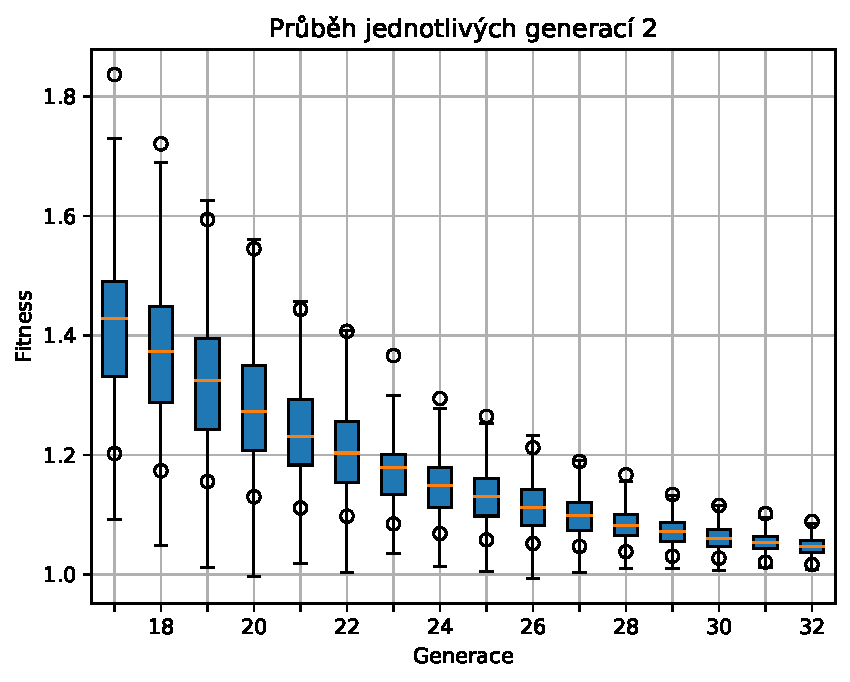
\includegraphics[width=75mm]{obrazky-figures/statistics/Benchmarks/Griewank/DE/evolutionProgress_1.pdf}
    &
	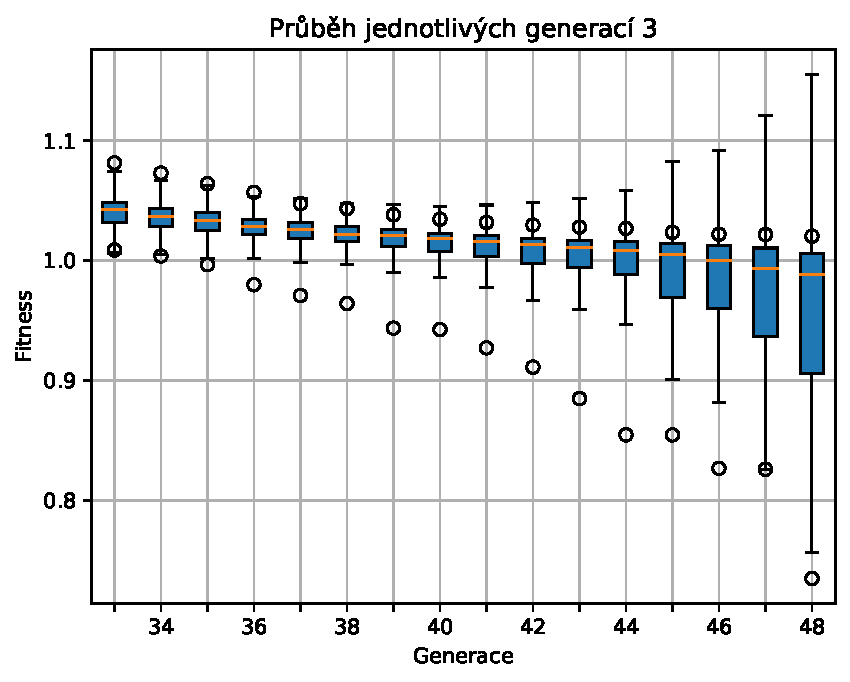
\includegraphics[width=75mm]{obrazky-figures/statistics/Benchmarks/Griewank/DE/evolutionProgress_2.pdf}
    &
	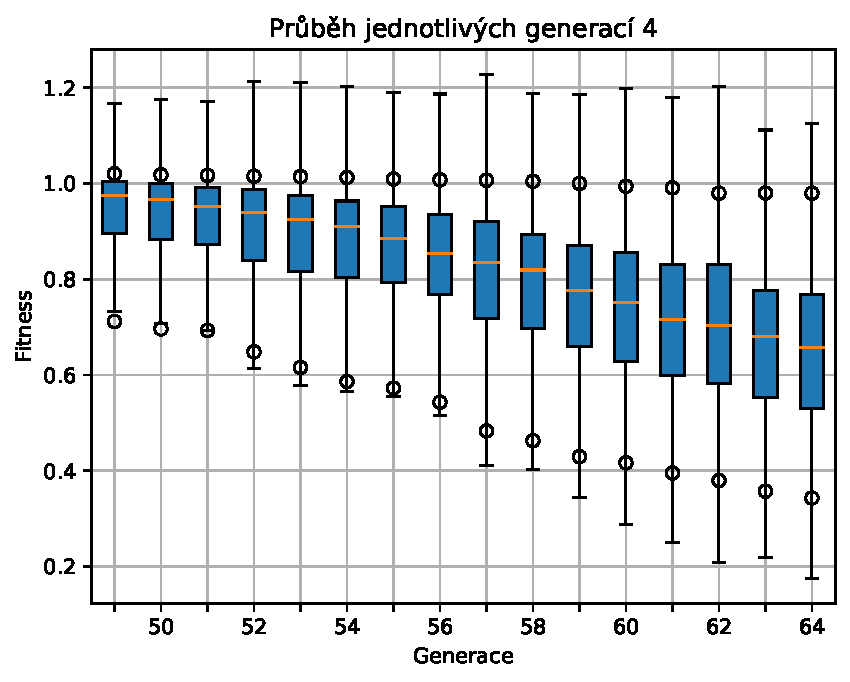
\includegraphics[width=75mm]{obrazky-figures/statistics/Benchmarks/Griewank/DE/evolutionProgress_3.pdf}
    \end{tabular}
    }
    \caption{Evoluční průběh DE. Data jsou mediány ze všech běhů v konkrétních generacích. Graf rozdělen na čtvrtiny pro větší detail. Body ukazují medián nejlepších a nejhorších nalezených řešení v dané generaci.}
    \label{fg:bench:griewank:de:evoProg}
\end{figure}

\subsubsection{Optimalizace rojem částic}
Pro nejoptimálnější řešení byly nalezeny parametry 
\begin{itemize}
    \item Velikost populace - $75$.
    \item Akcelerační koeficienty $c1 = c2 =2$.
    \item Váhový faktor setrvačnosti $0.5$.
    \item Roj s úplnou topologií.
\end{itemize}
Počet generací nadhodnocen, aby zastavení proběhlo nalezením optima nebo dosažením maximálního množství vyhodnocení fitness.

\begin{figure}[H]
\begin{minipage}[t]{0.475\linewidth}
\includegraphics[width=\linewidth]{obrazky-figures/statistics/Benchmarks/Griewank/PSO/bestsBoxplot_WithOutliers.pdf}
\caption{Boxplot nejlepších výsledků všech $30$ běhů PSO.}
\label{fg:bench:griewank:pso:best}
\end{minipage}
\hfill
\begin{minipage}[t]{0.475\linewidth}
\includegraphics[width=\linewidth]{obrazky-figures/statistics/Benchmarks/Griewank/PSO/lastGenBoxplots.pdf}
\caption{Boxplot stavu poslední generace všech $30$ běhů PSO.}
\label{fg:bench:griewank:pso:lastGen}
\end{minipage}
\end{figure}

\begin{figure}[H]
    \makebox[\textwidth][c]{
    \begin{tabular}{cc}
	\includegraphics[width=75mm]{obrazky-figures/statistics/Benchmarks/Griewank/PSO/evolutionProgress_0.pdf}
    &
	\includegraphics[width=75mm]{obrazky-figures/statistics/Benchmarks/Griewank/PSO/evolutionProgress_1.pdf}
    &
	\includegraphics[width=75mm]{obrazky-figures/statistics/Benchmarks/Griewank/PSO/evolutionProgress_2.pdf}
    &
	\includegraphics[width=75mm]{obrazky-figures/statistics/Benchmarks/Griewank/PSO/evolutionProgress_3.pdf}
    \end{tabular}
    }
    \caption{Evoluční průběh PSO. Data jsou mediány ze všech běhů v konkrétních generacích. Graf rozdělen na čtvrtiny pro větší detail. Body ukazují medián nejlepších a nejhorších nalezených řešení v dané generaci.}
    \label{fg:bench:griewank:pso:evoProg}
\end{figure}

\subsubsection{CMA-ES}
Výhodou \emph{CMA-ES} je skutečnost, že téměř všechny vstupní parametry jsou závislé pouze na dimenzi problému, který je předem daný. Maximální počet generací nadhodnocen, aby zastavení proběhlo nalezením optima nebo dosažením maximálního množství vyhodnocení fitness. Počáteční průměrná hodnota byla určena jako střední hodnota v mezích proměnných, standardní odchylka jako třetina absolutní hodnoty tohoto rozmezí.

\begin{figure}[H]
\begin{minipage}[t]{0.475\linewidth}
\includegraphics[width=\linewidth]{obrazky-figures/statistics/Benchmarks/Griewank/CMAES/bestsBoxplot_WithOutliers.pdf}
\caption{Boxplot nejlepších výsledků všech $30$ běhů CMA-ES.}
\label{fg:bench:griewank:pso:best}
\end{minipage}
\hfill
\begin{minipage}[t]{0.475\linewidth}
\includegraphics[width=\linewidth]{obrazky-figures/statistics/Benchmarks/Griewank/CMAES/lastGenBoxplots.pdf}
\caption{Boxplot stavu poslední generace všech $30$ běhů CMA-ES.}
\label{fg:bench:griewank:pso:lastGen}
\end{minipage}
\end{figure}

\begin{figure}[H]
    \makebox[\textwidth][c]{
    \begin{tabular}{cc}
	\includegraphics[width=75mm]{obrazky-figures/statistics/Benchmarks/Griewank/CMAES/evolutionProgress_0.pdf}
    &
	\includegraphics[width=75mm]{obrazky-figures/statistics/Benchmarks/Griewank/CMAES/evolutionProgress_1.pdf}
    &
	\includegraphics[width=75mm]{obrazky-figures/statistics/Benchmarks/Griewank/CMAES/evolutionProgress_2.pdf}
    &
	\includegraphics[width=75mm]{obrazky-figures/statistics/Benchmarks/Griewank/CMAES/evolutionProgress_3.pdf}
    \end{tabular}
    }
    \caption{Evoluční průběh CMA-ES. Data jsou mediány ze všech běhů v konkrétních generacích. Graf rozdělen na čtvrtiny pro větší detail. Body ukazují medián nejlepších a nejhorších nalezených řešení v dané generaci.}
    \label{fg:bench:griewank:pso:evoProg}
\end{figure}


\subsection{Rosenbrockova funkce}
\label{app:bench:rosen}

Následující grafy jsou kolekcí výsledků $30$ běhů každého optimalizačního algoritmu.
\subsubsection{Genetický algoritmus}
Pro optimalizaci byly použity následující parametry:
\begin{itemize}
    \item Velikost populace - $64$.
    \item Turnajový výběr.
    \item Dvoubodové křížení - $80\%$
    \item Mutace - $5\%$
    \item Vždy přežívají nejlepší řešení bez ohledu na to, ze které generace pochází.
\end{itemize}
Vzhledem k omezení na maximální počet evaluací byl počet generací fixně nadhodnocen, aby nebyl nikdy důvodem k zastavení algoritmu. 

\begin{figure}[H]
\begin{minipage}[t]{0.475\linewidth}
\includegraphics[width=\linewidth]{obrazky-figures/statistics/Benchmarks/Rosenbrock/GA/bestsBoxplot_WithOutliers.pdf}
\caption{Boxplot nejlepších výsledků všech $30$ běhů GA.}
\label{fg:bench:rosenbrock:ga:best}
\end{minipage}
\hfill
\begin{minipage}[t]{0.475\linewidth}
\includegraphics[width=\linewidth]{obrazky-figures/statistics/Benchmarks/Rosenbrock/GA/lastGenBoxplots.pdf}
\caption{Boxplot stavu poslední generace všech $30$ běhů GA.}
\label{fg:bench:rosenbrock:ga:lastGen}
\end{minipage}
\end{figure}

\begin{figure}[H]
    \makebox[\textwidth][c]{
    \begin{tabular}{cc}
	\includegraphics[width=75mm]{obrazky-figures/statistics/Benchmarks/Rosenbrock/GA/evolutionProgress_0.pdf}
    &
	\includegraphics[width=75mm]{obrazky-figures/statistics/Benchmarks/Rosenbrock/GA/evolutionProgress_1.pdf}
    &
	\includegraphics[width=75mm]{obrazky-figures/statistics/Benchmarks/Rosenbrock/GA/evolutionProgress_2.pdf}
    &
	\includegraphics[width=75mm]{obrazky-figures/statistics/Benchmarks/Rosenbrock/GA/evolutionProgress_3.pdf}
    \end{tabular}
    }
    \caption{Evoluční průběh GA. Data jsou mediány ze všech běhů v konkrétních generacích. Graf rozdělen na čtvrtiny pro větší detail. Body ukazují medián nejlepších a nejhorších nalezených řešení v dané generaci.}
    \label{fg:bench:rosenbrock:ga:evoProg}
\end{figure}


\subsubsection{Simulované žíhání}
Pro optimalizace řešení byly zvoleny následující parametry:
\begin{itemize}
    \item Počáteční teplota $2000$.
    \item Chladící krok $1\%$.
\end{itemize}
Teplotní rozvrh byl zvolen jako lineární. Perturberance maximálně o pětinu rozsahu.

\begin{figure}[H]
\begin{minipage}[t]{0.475\linewidth}
\includegraphics[width=\linewidth]{obrazky-figures/statistics/Benchmarks/Rosenbrock/SA/bestsBoxplot_WithOutliers.pdf}
\caption{Boxplot nejlepších výsledků všech $30$ běhů SA.}
\label{fg:bench:rosenbrock:sa:best}
\end{minipage}
\hfill
\begin{minipage}[t]{0.475\linewidth}
\includegraphics[width=\linewidth]{obrazky-figures/statistics/Benchmarks/Rosenbrock/SA/lastGenBoxplots.pdf}
\caption{Boxplot stavu poslední generace všech $30$ běhů SA.}
\label{fg:bench:rosenbrock:sa:lastGen}
\end{minipage}
\end{figure}

\subsubsection{Tabu prohledávání}
Optimalizace spouštěna s těmito parametry:
\begin{itemize}
    \item Velikost tabu seznamu - $20$.
    \item Velikost prohledávaného sousedství - $5$.
\end{itemize}
Využita byla pouze dlouhodobá paměť.

\begin{figure}[H]
\begin{minipage}[t]{0.475\linewidth}
\includegraphics[width=\linewidth]{obrazky-figures/statistics/Benchmarks/Rosenbrock/TABU/bestsBoxplot_WithOutliers.pdf}
\caption{Boxplot nejlepších výsledků všech $30$ běhů tabu prohledávání.}
\label{fg:bench:rosenbrock:tabu:best}
\end{minipage}
\hfill
\begin{minipage}[t]{0.475\linewidth}
\includegraphics[width=\linewidth]{obrazky-figures/statistics/Benchmarks/Rosenbrock/TABU/lastGenBoxplots.pdf}
\caption{Boxplot stavu poslední generace všech $30$ běhů tabu prohledávání.}
\label{fg:bench:rosenbrock:tabu:lastGen}
\end{minipage}
\end{figure}

\subsubsection{Diferenciální evoluce}
Pro optimalizaci byly použity tyto parametry:
\begin{itemize}
    \item Velikost populace - $30$.
    \item Rekombinace - $80\%$.
    \item Strategie \emph{best/1/bin}.
    \item Faktor zesílení $0.5$ až $0.7$.
\end{itemize}
I zde byl počet generací nadhodnocen tak, aby zastavení proběhlo nalezením optima nebo dosažením maximálního množství vyhodnocení fitness.

\begin{figure}[H]
\begin{minipage}[t]{0.475\linewidth}
\includegraphics[width=\linewidth]{obrazky-figures/statistics/Benchmarks/Rosenbrock/DE/bestsBoxplot_WithOutliers.pdf}
\caption{Boxplot nejlepších výsledků všech $30$ běhů DE.}
\label{fg:bench:rosenbrock:de:best}
\end{minipage}
\hfill
\begin{minipage}[t]{0.475\linewidth}
\includegraphics[width=\linewidth]{obrazky-figures/statistics/Benchmarks/Rosenbrock/DE/lastGenBoxplots.pdf}
\caption{Boxplot stavu poslední generace všech $30$ DE.}
\label{fg:bench:rosenbrock:de:lastGen}
\end{minipage}
\end{figure}

\begin{figure}[H]
    \makebox[\textwidth][c]{
    \begin{tabular}{cc}
	\includegraphics[width=75mm]{obrazky-figures/statistics/Benchmarks/Rosenbrock/DE/evolutionProgress_0.pdf}
    &
	\includegraphics[width=75mm]{obrazky-figures/statistics/Benchmarks/Rosenbrock/DE/evolutionProgress_1.pdf}
    &
	\includegraphics[width=75mm]{obrazky-figures/statistics/Benchmarks/Rosenbrock/DE/evolutionProgress_2.pdf}
    &
	\includegraphics[width=75mm]{obrazky-figures/statistics/Benchmarks/Rosenbrock/DE/evolutionProgress_3.pdf}
    \end{tabular}
    }
    \caption{Evoluční průběh DE. Data jsou mediány ze všech běhů v konkrétních generacích. Graf rozdělen na čtvrtiny pro větší detail. Body ukazují medián nejlepších a nejhorších nalezených řešení v dané generaci.}
    \label{fg:bench:rosenbrock:de:evoProg}
\end{figure}


\subsubsection{Optimalizace rojem částic}
Pro nejoptimálnější řešení byly nalezeny parametry 
\begin{itemize}
    \item $75$ částic v roji.
    \item Akcelerační koeficienty $c1 = c2 = 1$ 
    \item Váhový faktor akcelerace - $0.5$
\end{itemize}
Počet generací nadhodnocen, aby zastavení proběhlo nalezením optima nebo dosažením maximálního množství vyhodnocení fitness.

\begin{figure}[H]
\begin{minipage}[t]{0.475\linewidth}
\includegraphics[width=\linewidth]{obrazky-figures/statistics/Benchmarks/Rosenbrock/PSO/bestsBoxplot_WithOutliers.pdf}
\caption{Boxplot nejlepších výsledků všech $30$ běhů PSO.}
\label{fg:bench:rosenbrock:pso:best}
\end{minipage}
\hfill
\begin{minipage}[t]{0.475\linewidth}
\includegraphics[width=\linewidth]{obrazky-figures/statistics/Benchmarks/Rosenbrock/PSO/lastGenBoxplots.pdf}
\caption{Boxplot stavu poslední generace všech $30$ PSO.}
\label{fg:bench:rosenbrock:pso:lastGen}
\end{minipage}
\end{figure}

\begin{figure}[H]
    \makebox[\textwidth][c]{
    \begin{tabular}{cc}
	\includegraphics[width=75mm]{obrazky-figures/statistics/Benchmarks/Rosenbrock/PSO/evolutionProgress_0.pdf}
    &
	\includegraphics[width=75mm]{obrazky-figures/statistics/Benchmarks/Rosenbrock/PSO/evolutionProgress_1.pdf}
    &
	\includegraphics[width=75mm]{obrazky-figures/statistics/Benchmarks/Rosenbrock/PSO/evolutionProgress_2.pdf}
    &
	\includegraphics[width=75mm]{obrazky-figures/statistics/Benchmarks/Rosenbrock/PSO/evolutionProgress_3.pdf}
    \end{tabular}
    }
    \caption{Evoluční průběh PSO. Data jsou mediány ze všech běhů v konkrétních generacích. Graf rozdělen na čtvrtiny pro větší detail. Body ukazují medián nejlepších a nejhorších nalezených řešení v dané generaci.}
    \label{fg:bench:rosenbrock:pso:evoProg}
\end{figure}

\subsubsection{CMA-ES}
Výhodou \emph{CMA-ES} je skutečnost, že téměř všechny vstupní parametry jsou závislé pouze na dimenzi problému, který je předem daný. Maximální počet generací nadhodnocen, aby zastavení proběhlo nalezením optima nebo dosažením maximálního množství vyhodnocení fitness. Počáteční průměrná hodnota byla určena jako střední hodnota v mezích proměnných, standardní odchylka jako třetina absolutní hodnoty tohoto rozmezí.

\begin{figure}[H]
\begin{minipage}[t]{0.475\linewidth}
\includegraphics[width=\linewidth]{obrazky-figures/statistics/Benchmarks/Rosenbrock/CMAES/bestsBoxplot_WithOutliers.pdf}
\caption{Boxplot nejlepších výsledků všech $30$ běhů CMA-ES.}
\label{fg:bench:rosenbrock:cmaes:best}
\end{minipage}
\hfill
\begin{minipage}[t]{0.475\linewidth}
\includegraphics[width=\linewidth]{obrazky-figures/statistics/Benchmarks/Rosenbrock/CMAES/lastGenBoxplots.pdf}
\caption{Boxplot stavu poslední generace všech $30$ CMA-ES.}
\label{fg:bench:rosenbrock:cmaes:lastGen}
\end{minipage}
\end{figure}

\begin{figure}[H]
    \makebox[\textwidth][c]{
    \begin{tabular}{cc}
	\includegraphics[width=75mm]{obrazky-figures/statistics/Benchmarks/Rosenbrock/CMAES/evolutionProgress_0.pdf}
    &
	\includegraphics[width=75mm]{obrazky-figures/statistics/Benchmarks/Rosenbrock/CMAES/evolutionProgress_1.pdf}
    &
	\includegraphics[width=75mm]{obrazky-figures/statistics/Benchmarks/Rosenbrock/CMAES/evolutionProgress_2.pdf}
    &
	\includegraphics[width=75mm]{obrazky-figures/statistics/Benchmarks/Rosenbrock/CMAES/evolutionProgress_3.pdf}
    \end{tabular}
    }
    \caption{Evoluční průběh CMA-ES. Data jsou mediány ze všech běhů v konkrétních generacích. Graf rozdělen na čtvrtiny pro větší detail. Body ukazují medián nejlepších a nejhorších nalezených řešení v dané generaci.}
    \label{fg:bench:rosenbrock:cmaes:evoProg}
\end{figure}

\chapter{Vizualizace výsledků hledání HIFU trajektorie}
Tato kapitola detailně zobrazuje nalezená nejlepší řešení při hledání trajektorie HIFU sonikací.

\section{Skvrna - malý počet sonikací}
Obrázek \ref{fg:hifu:prog} vizualizuje průběh simulace nejlepší nalezené trajektorie nad modelem skvrna o $4$ sonikacích. Nejlepší nalezená trajektorie $I_{best}$ skončila simulaci s následujícími výsledky:
\begin{center}
\begin{itemize}
    \item $0.30349\%$ cílené tkáně přežilo - $3$ body matice
    \item $0.0071788\%$ necílené tkáně bylo zničeno - $1$ bod matice
\end{itemize}
\end{center}


\begin{figure}[H]
    \makebox[\textwidth][c]{
    \begin{tabular}{}
	\includegraphics[width=\linewidth]{obrazky-figures/hifuSimProgress/blob20/blob20_0_croped.pdf}
	&
	\includegraphics[width=\linewidth]{obrazky-figures/hifuSimProgress/son1.pdf}
    &
	\includegraphics[width=\linewidth]{obrazky-figures/hifuSimProgress/son2.pdf}
    &
	\includegraphics[width=\linewidth]{obrazky-figures/hifuSimProgress/son3.pdf}
    &
	\includegraphics[width=\linewidth]{obrazky-figures/hifuSimProgress/son4.pdf}
    \end{tabular}
    }
    \caption{Postupný průběh simulace nejlepšího nalezeného řešení. První řádek ukazuje počáteční stav modelu, každý další řádek poté reprezentuje stav po provedení jedné sonikace. Levý sloupec zobrazuje tkáň, která nebyla cílena a přesto proběhla ablace (při poslední sonikaci byl zasažen jeden bod, proto došlo ke změně kontury bez zřejmého důvodu). Prostřední sloupec ukazuje cílenou tkáň, která je stále naživu. Pravý sloupec ukazuje zničenou oblast na pozadí CT snímku použitého média.}
    \label{fg:hifu:prog}
\end{figure}


\section{Skvrna - velký počet sonikací}
Obrázek \ref{fg:hifu:blob:prog} vizualizuje průběh simulace nejlepší nalezené trajektorie nad modelem skvrna o $20$ sonikacích. Nejlepší nalezená trajektorie $I_{best}$ skončila simulaci s následujícími výsledky:
\begin{center}
\begin{itemize}
    \item $0\%$ cílené tkáně přežilo
    \item $0.035894\%$ necílené tkáně bylo zničeno - $5$ bodů matice
\end{itemize}
\end{center}


\begin{figure}[H]
    \makebox[\textwidth][c]{
    \begin{tabular}{}
	\includegraphics[width=\linewidth]{obrazky-figures/hifuSimProgress/blob20/blob20_0_croped.pdf}
    &
	\includegraphics[width=\linewidth]{obrazky-figures/hifuSimProgress/blob20/blob20_5_croped.pdf}
    &
	\includegraphics[width=\linewidth]{obrazky-figures/hifuSimProgress/blob20/blob20_10_croped.pdf}
    &
	\includegraphics[width=\linewidth]{obrazky-figures/hifuSimProgress/blob20/blob20_15_croped.pdf}
    &
	\includegraphics[width=\linewidth]{obrazky-figures/hifuSimProgress/blob20/blob20_20_croped.pdf}
    \end{tabular}
    }
    \caption{Postupný průběh simulace nejlepšího nalezeného řešení HIFU operace. První řádek ukazuje stav modelu před začátkem operace, každý další řádek poté reprezentuje stav modelu po provedení následujících $5$ti sonikací. Levý sloupec zobrazuje tkáň, která nebyla cílena a přesto proběhla ablace (při poslední sonikaci byl zasaženo několik bod, proto došlo ke změně kontury bez zřejmého důvodu). Prostřední sloupec ukazuje cílenou tkáň, která je stále naživu. Pravý sloupec ukazuje zničenou oblast na pozadí CT snímku použitého média.}
    \label{fg:hifu:blob:prog}
\end{figure}


\section{Květina}
Obrázek \ref{fg:hifu:flower:prog} vizualizuje průběh simulace nejlepší nalezené trajektorie nad modelem skvrna o $20$ sonikacích. Nejlepší nalezená trajektorie $I_{best}$ skončila simulaci s následujícími výsledky:
\begin{center}
\begin{itemize}
    \item $2.7664\%$ cílené tkáně přežilo - $108$ bodů matice
    \item $0.36112\%$ necílené tkáně bylo zničeno - $160$ bodů matice
\end{itemize}
\end{center}


\begin{figure}[H]
    \makebox[\textwidth][c]{
    \begin{tabular}{}
	\includegraphics[width=\linewidth]{obrazky-figures/hifuSimProgress/flower15/flower15_0_croped.pdf}
    &
    	\includegraphics[width=\linewidth]{obrazky-figures/hifuSimProgress/flower15/flower15_5_croped.pdf}
    &
    	\includegraphics[width=\linewidth]{obrazky-figures/hifuSimProgress/flower15/flower15_10_croped.pdf}
    &
    	\includegraphics[width=\linewidth]{obrazky-figures/hifuSimProgress/flower15/flower15_15_croped.pdf}
    &
    \end{tabular}
    }
    \caption{Postupný průběh simulace nejlepšího nalezeného řešení HIFU operace. První řádek je počáteční stav modelu před začátkem operace, každý další řádek reprezentuje provedení následujících $5$ti sonikací. Levý sloupec zobrazuje tkáň, která nebyla cílena a přesto proběhla ablace. Prostřední sloupec ukazuje cílenou tkáň, která je stále naživu. Pravý sloupec ukazuje zničenou oblast na pozadí CT snímku použitého média.}
    \label{fg:hifu:flower:prog}
\end{figure}